% ============================================================
%  يُترجَم بـ XeLaTeX  (في Overleaf: Menu → Compiler → XeLaTeX)
%  الخط: Amiri (متوفر في Overleaf، أو حمّله من github.com/aliftype/amiri)
% ============================================================
\documentclass[12pt,a4paper]{article}
\usepackage[a4paper,margin=1.7cm,top=2.3cm,bottom=2.9cm,headheight=15pt,footskip=1.5cm]{geometry}
\usepackage{amsmath,amssymb}
\usepackage{icomma}
\usepackage[english,bidi=default,layout=lists]{babel}
\babelprovide[import,main]{arabic}
\babelfont{rm}[Scale=1.08]{Amiri}
\babelfont{sf}[Scale=1.08]{Amiri}
\usepackage[most]{tcolorbox}
\usepackage{tikz}
\usetikzlibrary{arrows.meta,calc,shadings}
\usepackage{array}
\usepackage{colortbl}
\usepackage{fancyhdr}
\usepackage{titlesec}
\usepackage{enumitem}
\usepackage{collcell}
\usepackage{needspace}
\usepackage{etoolbox}
% أعمدة جداول تُكتب خلاياها بالعربية في الاتجاه الصحيح
\newcolumntype{C}{>{\collectcell\ar}c<{\endcollectcell}}
% تجنب عنوان يتيم في أسفل الصفحة
\pretocmd{\section}{\Needspace{15\baselineskip}}{}{}
\pretocmd{\subsection}{\Needspace{11\baselineskip}}{}{}

% ---------- الألوان ----------
\definecolor{cDef}{HTML}{1F4E9C}
\definecolor{cThm}{HTML}{B3261E}
\definecolor{cRem}{HTML}{2E7D32}
\definecolor{cEx}{HTML}{C76B00}
\definecolor{cMeth}{HTML}{6A1B9A}
\definecolor{cSol}{HTML}{00695C}
\definecolor{cSec}{HTML}{1F3A68}

% ---------- العناوين ----------
\titleformat{\section}{\Large\bfseries\color{cSec}}{\thesection.}{0.6em}{}[{\color{cSec!60}\titlerule[1pt]}]
\titleformat{\subsection}{\large\bfseries\color{cThm!85!black}}{\thesubsection.}{0.5em}{}
\titlespacing*{\section}{0pt}{14pt}{8pt}
\titlespacing*{\subsection}{0pt}{10pt}{5pt}
\setlength{\parindent}{0pt}
\setlength{\parskip}{4pt}
\setlist{itemsep=2pt,topsep=3pt}

% ---------- الصناديق (تُرسم في سياق LTR ويُكتب محتواها بالعربية) ----------
\newtcolorbox{arbox}[3][]{enhanced,
  colback=#2!5,colframe=#2!80!black,arc=2mm,boxrule=0.8pt,
  left=6pt,right=6pt,top=8pt,bottom=5pt,
  fonttitle=\bfseries,coltitle=white,
  title={\foreignlanguage{arabic}{#3}},
  attach boxed title to top right={xshift=-5mm,yshift=-3mm},
  boxed title style={colback=#2!80!black,arc=1.5mm,boxrule=0pt},
  before upper={\selectlanguage{arabic}},
  before skip=8pt,after skip=8pt,breakable,#1}
\newenvironment{BOX}[2]{\begin{otherlanguage}{english}\begin{arbox}{#1}{#2}}{\end{arbox}\end{otherlanguage}}
\newenvironment{tarif}[1][تعريف]{\begin{BOX}{cDef}{#1}}{\end{BOX}}
\newenvironment{khassia}[1][خاصية]{\begin{BOX}{cThm}{#1}}{\end{BOX}}
\newenvironment{molahada}[1][ملاحظة]{\begin{BOX}{cRem}{#1}}{\end{BOX}}
\newenvironment{mithal}[1][مثال]{\begin{BOX}{cEx}{#1}}{\end{BOX}}
\newenvironment{tariqa}[1][طريقة]{\begin{BOX}{cMeth}{#1}}{\end{BOX}}

% ---------- التمارين والحلول ----------
\newcounter{exo}
\newenvironment{tamrin}[1]{\stepcounter{exo}\begin{BOX}{cSec}{التمرين \theexo: #1}}{\end{BOX}}
\newenvironment{hal}{\Needspace{12\baselineskip}\begin{otherlanguage}{english}\begin{arbox}[breakable]{cSol}{حل التمرين \theexo}}{\end{arbox}\end{otherlanguage}}

% رسومات TikZ تُوضع في سياق LTR
\newenvironment{LTR}{\begin{otherlanguage}{english}}{\end{otherlanguage}}
\newcommand{\ar}[1]{\foreignlanguage{arabic}{#1}}

% ---------- رموز ----------
% نقاط الحذف داخل الرياضيات (\dots يسبب خللاً في الاتجاه مع babel)
\renewcommand{\dots}{\mathinner{\ldotp\ldotp\ldotp}}
\renewcommand{\ldots}{\mathinner{\ldotp\ldotp\ldotp}}
\renewcommand{\cdots}{\mathinner{\cdotp\cdotp\cdotp}}
\newcommand{\N}{\mathbb{N}}
\newcommand{\Z}{\mathbb{Z}}
\newcommand{\D}{\mathbb{D}}
\newcommand{\Q}{\mathbb{Q}}
\newcommand{\R}{\mathbb{R}}
\newcommand{\pgcd}{\operatorname{PGCD}}
\newcommand{\ppcm}{\operatorname{PPCM}}

% ---------- تمثيل مجال على مستقيم عددي ----------
% \NLseg{a}{b}{[}{]}  مجال محدود
\newcommand{\NLseg}[4]{\begin{LTR}\begin{tikzpicture}[baseline=-0.6ex]
 \draw[-{Stealth[length=2mm]},gray!70](0,0)--(3.4,0);
 \draw[line width=2pt,cThm!80!black](0.7,0)--(2.7,0);
 \node[cThm!80!black,font=\LARGE] at (0.7,0){$#3$};
 \node[cThm!80!black,font=\LARGE] at (2.7,0){$#4$};
 \node[below=3pt,font=\footnotesize] at (0.7,0){$#1$};
 \node[below=3pt,font=\footnotesize] at (2.7,0){$#2$};
\end{tikzpicture}\end{LTR}}
% \NLright{a}{[}  مجال نحو +∞
\newcommand{\NLright}[2]{\begin{LTR}\begin{tikzpicture}[baseline=-0.6ex]
 \draw[-{Stealth[length=2mm]},gray!70](0,0)--(3.4,0);
 \draw[line width=2pt,cThm!80!black](1.3,0)--(3.3,0);
 \node[cThm!80!black,font=\LARGE] at (1.3,0){$#2$};
 \node[below=3pt,font=\footnotesize] at (1.3,0){$#1$};
\end{tikzpicture}\end{LTR}}
% \NLleft{b}{]}  مجال نحو −∞
\newcommand{\NLleft}[2]{\begin{LTR}\begin{tikzpicture}[baseline=-0.6ex]
 \draw[-{Stealth[length=2mm]},gray!70](0,0)--(3.4,0);
 \draw[line width=2pt,cThm!80!black](0.05,0)--(2.1,0);
 \node[cThm!80!black,font=\LARGE] at (2.1,0){$#2$};
 \node[below=3pt,font=\footnotesize] at (2.1,0){$#1$};
\end{tikzpicture}\end{LTR}}

% ---------- أيقونات مواقع التواصل (مرسومة بـ TikZ، لا تحتاج أي حزمة) ----------
\definecolor{cFB}{HTML}{1877F2}
\definecolor{cTG}{HTML}{229ED9}
\definecolor{cIG1}{HTML}{FEDA75}
\definecolor{cIG2}{HTML}{D62976}
\definecolor{cIG3}{HTML}{4F5BD5}
\newcommand{\fbicon}{\begin{LTR}\begin{tikzpicture}[baseline=-0.75ex,x=1em,y=1em]
 \fill[cFB] (0,0) circle (0.55);
 \node[white,inner sep=0,font=\usefont{TU}{lmss}{bx}{n}\small] at (0.04,-0.02) {f};
\end{tikzpicture}\end{LTR}}
\newcommand{\igicon}{\begin{LTR}
\begin{tikzpicture}[baseline=-0.75ex,x=1em,y=1em]
 \shade[lower left=cIG1,lower right=cIG2,upper left=cIG2,upper right=cIG3,rounded corners=0.28em] (-0.55,-0.55) rectangle (0.55,0.55);
 \draw[white,line width=0.09em,rounded corners=0.18em] (-0.36,-0.36) rectangle (0.36,0.36);
 \draw[white,line width=0.09em] (0,0) circle (0.17);
 \fill[white] (0.22,0.22) circle (0.05);
\end{tikzpicture}\end{LTR}}
\newcommand{\tgicon}{\begin{LTR}
\begin{tikzpicture}[baseline=-0.75ex,x=1em,y=1em]
 \fill[cTG] (0,0) circle (0.55);
 \fill[white] (-0.33,0.0) -- (0.32,0.27) -- (0.2,-0.3) -- (0.0,-0.15) -- (-0.08,-0.28) -- (-0.08,-0.08) -- cycle;
 \fill[cTG!70!black] (-0.08,-0.08) -- (0.25,0.2) -- (0.0,-0.15) -- (-0.08,-0.28) -- cycle;
\end{tikzpicture}\end{LTR}}
% سطر مواقع التواصل أسفل كل صفحة
% (يُكتب السطر بترتيب بصري من اليسار إلى اليمين: الأيقونة يمين كل اسم)
\newcommand{\PageBox}{\begin{LTR}\tikz[baseline=(p.base)]\node[fill=black,text=white,inner sep=2.5pt,minimum width=1.6em,minimum height=1.3em,font=\usefont{TU}{lmss}{bx}{n}\small](p){\ifnum\value{page}<10 0\fi\arabic{page}};\end{LTR}}
\newcommand{\SocialRow}{\begin{otherlanguage}{english}%
 \ar{\textbf{الأستاذ سوايسية هشام للرياضيات}}\ \tgicon\hfill
 \textbf{prof\_hicham\_math}\ \igicon\hfill
 \ar{\textbf{الأستاذ سوايسية هشام للرياضيات}}\ \fbicon\hspace{2.2em}\PageBox\end{otherlanguage}}
% ---------- رأس وتذييل الصفحة ----------
\pagestyle{fancy}
\fancyhf{}
\renewcommand{\headrulewidth}{0.6pt}
\renewcommand{\footrulewidth}{0.4pt}
% \SetHeader{يمين الرأس}{يسار الرأس}{يمين التذييل}{يسار التذييل}
\newcommand{\SetHeader}[2]{%
 \fancyhead[C]{\parbox{\textwidth}{\ar{#1\hfill #2}}}%
 \fancyfoot[C]{\parbox{\textwidth}{\small\SocialRow}}}

\usepackage{tkz-tab}
\usepackage{multicol}
% جدول تغيرات / إشارة (يُرسم في سياق LTR)
\newenvironment{TAB}{\par\begin{center}\begin{LTR}\begin{tikzpicture}[scale=0.95,every node/.style={font=\small}]}{\end{tikzpicture}\end{LTR}\end{center}}
% معلم بشبكة: \begin{GR}{xmin}{xmax}{ymin}{ymax}{unit cm}
\newenvironment{GR}[5]{\par\begin{center}\begin{LTR}\begin{tikzpicture}[x=#5cm,y=#5cm,font=\footnotesize]
 \def\xmn{#1}\def\xmx{#2}\def\ymn{#3}\def\ymx{#4}
 \draw[gray!25,very thin] (#1,#3) grid (#2,#4);
 \draw[-{Stealth[length=2mm]}] (#1,0)--(#2+0.3,0) node[below left]{$x$};
 \draw[-{Stealth[length=2mm]}] (0,#3)--(0,#4+0.3) node[below left]{$y$};
 \node[below left] at (0,0){$O$};
 \draw[very thick,-{Stealth[length=1.6mm]}] (0,0)--(1,0) node[below,pos=.55]{$\vec i$};
 \draw[very thick,-{Stealth[length=1.6mm]}] (0,0)--(0,1) node[left,pos=.55]{$\vec j$};
 \begin{scope}\clip (#1,#3) rectangle (#2,#4);}
{\end{scope}\end{tikzpicture}\end{LTR}\end{center}}
\newcommand{\Ticks}[2]{\foreach \t in {#1} \node[below,font=\scriptsize] at (\t,0){$\t$}; \foreach \t in {#2} \node[left,font=\scriptsize] at (0,\t){$\t$};}
\newcommand{\bx}[1]{\ensuremath{\colorbox{cDef!12}{$\displaystyle #1$}}}
\newcommand{\hl}[1]{\ensuremath{\colorbox{cEx!20}{$\displaystyle #1$}}}
\newcommand{\Lim}[1]{\displaystyle\lim_{x\to #1}}
\newcommand{\Cf}{(C_f)}
\newenvironment{qst}{\begin{enumerate}[label=\protect\circled{\arabic*},leftmargin=*]}{\end{enumerate}}
\newcommand{\circled}[1]{\foreignlanguage{english}{\tikz[baseline=(c.base)]\node[circle,fill=cDef,text=white,inner sep=1.2pt,font=\scriptsize\bfseries](c){#1};}}
% عمودان: \TwoCol{عرض اليسار}{محتوى اليسار}{عرض اليمين}{محتوى اليمين}  (آمن مع TikZ)
\newcommand{\TwoCol}[4]{\par\begin{LTR}\noindent\begin{minipage}[t]{#1\textwidth}\selectlanguage{arabic}#2\end{minipage}\hfill\begin{minipage}[t]{#3\textwidth}\selectlanguage{arabic}#4\end{minipage}\end{LTR}\par}
\newcommand{\un}{(u_n)}\newcommand{\vn}{(v_n)}
% برهان بالتراجع: \Rec{الخاصية P(n)}{التحقق من P(0)}{البرهان على الوراثة}
\newcommand{\Rec}[3]{\textbf{برهان بالتراجع:} نسمي $P(n)$ الخاصية: «#1».
\begin{itemize}
\item \textbf{التحقق:} #2
\item \textbf{الوراثة:} نفرض أن $P(n)$ صحيحة ونبرهن صحة $P(n+1)$: #3
\item \textbf{الخلاصة:} حسب مبدأ الاستدلال بالتراجع، $P(n)$ صحيحة من أجل كل عدد طبيعي $n$.
\end{itemize}}
\newcommand{\src}[1]{{\footnotesize\textbf{#1}}\par}
\newcommand{\ok}{$\textcolor{cRem}{\checkmark}$}
\newcommand{\limn}{\displaystyle\lim_{n\to+\infty}}
% أسئلة فرعية (أ) (ب) (جـ) كل سؤال في سطر
\newenvironment{sq}{\begin{itemize}[leftmargin=2.4em,itemsep=3pt]}{\end{itemize}}
\newcommand{\qa}{\item[(أ)]}\newcommand{\qb}{\item[(ب)]}\newcommand{\qc}{\item[(جـ)]}\newcommand{\qd}{\item[(د)]}\newcommand{\qe}{\item[(هـ)]}
\newcommand{\pa}{\par\smallskip\textbf{(أ)} }\newcommand{\pb}{\par\smallskip\textbf{(ب)} }\newcommand{\pc}{\par\smallskip\textbf{(جـ)} }\newcommand{\pd}{\par\smallskip\textbf{(د)} }\newcommand{\pe}{\par\smallskip\textbf{(هـ)} }
\newcommand{\ccl}[1]{\par\textbf{الخلاصة:} #1}

\pretocmd{\section}{\Needspace{24\baselineskip}}{}{}
\newcommand{\RL}[4]{\TwoCol{#3}{#4}{#1}{#2}}
\renewcommand{\bx}[1]{\ensuremath{\colorbox{cDef!12}{$\displaystyle\color{cThm}#1$}}}
\newtcbox{\bxtbox}{on line,coltext=cThm,colback=cDef!12,colframe=cDef!12,boxrule=0pt,arc=1pt,boxsep=0pt,left=2pt,right=2pt,top=1pt,bottom=1pt}
\newcommand{\bxt}[1]{\foreignlanguage{english}{\bxtbox{\ar{#1}}}}
\newcommand{\LW}[1]{{\color{cDef}#1}}
\newcommand{\QQ}[1]{\par\smallskip\textbf{#1.} }
\newcommand{\ABC}[3]{\\[2pt]\begin{tabular}{p{0.28\textwidth}p{0.28\textwidth}p{0.28\textwidth}}(جـ) \ #3 & (ب) \ #2 & (أ) \ #1\end{tabular}}
\newcommand{\yes}{{\color{cRem}\checkmark}}
\newcommand{\no}{{\color{cThm}$\times$}}
\relpenalty=10000\binoppenalty=10000\tolerance=9000\emergencystretch=0.3\linewidth
\SetHeader{\small\bfseries\color{cSec}تمارين الوحدة الأولى: الأعداد والحساب}{\small\color{cSec}السنة الأولى ثانوي -- جذع مشترك علوم وتكنولوجيا}
\begin{document}
\begin{LTR}
\begin{tcolorbox}[enhanced,colback=cSec!10,colframe=cSec!40,arc=3mm,halign=center,boxrule=0.6pt,top=12pt,bottom=12pt,before upper={\selectlanguage{arabic}}]
{\color{cSec}\fontsize{25}{31}\selectfont\bfseries سلسلة تمارين: الأعداد والحساب}\\[8pt]
{\color{cSec!80!black}\large الوحدة الأولى: المجموعات ، الحساب ، الترتيب في $\mathbb{R}$ والقيمة المطلقة -- مع الحلول المفصلة}\\[5pt]
{\color{cSec!80!black}\large السنة الأولى ثانوي -- جذع مشترك علوم وتكنولوجيا}
\end{tcolorbox}
\end{LTR}

% =====================================================================
\section{مجموعات الأعداد والكتابة الكسرية}
\begin{tamrin}{مجموعات الأعداد}
\begin{enumerate}
\item انقل الجدول ثم أكمله بوضع العلامة \yes\ إذا كان العدد ينتمي إلى المجموعة ، والعلامة \no\ إذا كان لا ينتمي إليها.
\begin{center}
\renewcommand{\arraystretch}{1.6}
\begin{tabular}{|c|c|c|c|c|c|c|c|c|}\hline
\rowcolor{cSec!12}$\dfrac{22}7$ & $\pi$ & $10^{-2}$ & $-\sqrt5$ & $\dfrac23$ & $\sqrt{16}$ & $\dfrac74$ & $-3$ & \ar{العدد}\\\hline
 & & & & & & & & $\N$\\\hline
 & & & & & & & & $\Z$\\\hline
 & & & & & & & & $\D$\\\hline
 & & & & & & & & $\Q$\\\hline
 & & & & & & & & $\R$\\\hline
\end{tabular}
\end{center}
\item بيّن أن $\dfrac3{40}$ عدد عشري ، وأن $\dfrac13$ ليس عددًا عشريًا.
\end{enumerate}
\end{tamrin}
\begin{hal}
\textbf{1.} الجدول المكتمل:
\begin{center}
\renewcommand{\arraystretch}{1.6}
\begin{tabular}{|c|c|c|c|c|c|c|c|c|}\hline
\rowcolor{cSec!12}$\dfrac{22}7$ & $\pi$ & $10^{-2}=0{,}01$ & $-\sqrt5$ & $\dfrac23$ & $\sqrt{16}=4$ & $\dfrac74=1{,}75$ & $-3$ & \ar{العدد}\\\hline
\no & \no & \no & \no & \no & \yes & \no & \no & $\N$\\\hline
\no & \no & \no & \no & \no & \yes & \no & \yes & $\Z$\\\hline
\no & \no & \yes & \no & \no & \yes & \yes & \yes & $\D$\\\hline
\yes & \no & \yes & \no & \yes & \yes & \yes & \yes & $\Q$\\\hline
\yes & \yes & \yes & \yes & \yes & \yes & \yes & \yes & $\R$\\\hline
\end{tabular}
\end{center}
\textbf{تنبيه:} $\dfrac{22}7=3{,}142857\dots$ عدد ناطق وهو قيمة مقربة للعدد $\pi$ فقط ، و $\pi$ عدد أصم.
\QQ{2} $\dfrac3{40}=\dfrac{3\times25}{40\times25}=\dfrac{75}{1000}=\dfrac{75}{10^3}=0{,}075$ \quad إذن \quad \bx{\frac3{40}\in\D}\par
نفرض بالخلف أن $\dfrac13\in\D$ ، أي يوجد $a\in\Z$ و $n\in\N$ حيث $\dfrac13=\dfrac a{10^n}$ ، ومنه $3a=10^n=2^n\times5^n$.\par
إذن $3$ يقسم $2^n\times5^n$ ، وهذا مستحيل لأن العوامل الأولية لـ $10^n$ هي $2$ و $5$ فقط. \quad إذن \quad \bx{\frac13\notin\D}
\end{hal}

\begin{tamrin}{من الكتابة الدورية إلى الكتابة الكسرية}
اكتب كل عدد من الأعداد التالية على شكل كسر غير قابل للاختزال:
\[a=0{,}777\dots=0{,}\overline{7}\qquad;\qquad b=2{,}1515\dots=2{,}\overline{15}\qquad;\qquad c=0{,}12727\dots=0{,}1\overline{27}\]
\end{tamrin}
\begin{hal}
\textbf{1.} $a=0{,}\overline7$: دور من رقم واحد ، نضرب في $10$: \quad $10a=7+a$ \quad ومنه \quad $9a=7$ \quad أي \quad \bx{a=\frac79}
\QQ{2} $b=2+x$ حيث $x=0{,}\overline{15}$: دور من رقمين: \quad $100x=15+x$ \quad ومنه \quad $99x=15$ \quad أي \quad $x=\dfrac{15}{99}=\dfrac5{33}$\par
إذن: \quad $b=2+\dfrac5{33}=\bx{\frac{71}{33}}$
\QQ{3} $c=0{,}1\overline{27}$: \quad $10c=1{,}\overline{27}$ \quad و \quad $1000c=127{,}\overline{27}$\par
بالطرح: \quad $1000c-10c=127-1$ \quad أي \quad $990c=126$\par
ومنه: \quad $c=\dfrac{126}{990}=\bx{\frac7{55}}$ \quad (قسمنا البسط والمقام على $18=\pgcd(126;990)$). \quad تحقق: $7\div55=0{,}12727\dots$ \ok
\end{hal}

\begin{tamrin}{أصغر مجموعة ينتمي إليها عدد}
عيّن أصغر مجموعة من بين $\N$ ، $\Z$ ، $\D$ ، $\Q$ ، $\R$ ينتمي إليها كل عدد:
\[a=\sqrt{49}-10\quad;\quad b=\frac3{40}\quad;\quad c=\frac{14}{21}\quad;\quad d=\frac{\left(\sqrt5-1\right)\left(\sqrt5+1\right)}8\]
\[e=\sqrt2\left(1+\frac1{1+\sqrt2}\right)\quad;\quad f=-\frac\pi4\]
\end{tamrin}
\begin{hal}
\begin{itemize}
\item $a=7-10=-3$ \quad إذن \quad \bx{a\in\Z} \quad ($a\notin\N$).
\item $b=\dfrac3{2^3\times5}=0{,}075$ \quad إذن \quad \bx{b\in\D}
\item $c=\dfrac23$ (بعد الاختزال على $7$) والمقام $3$ \quad إذن \quad \bx{c\in\Q} \quad و $c\notin\D$.
\item $d=\dfrac{5-1}8=\dfrac12=0{,}5$ \quad إذن \quad \bx{d\in\D}
\item $\dfrac1{1+\sqrt2}=\dfrac{\sqrt2-1}{2-1}=\sqrt2-1$ ، ومنه $e=\sqrt2\left(1+\sqrt2-1\right)=\sqrt2\times\sqrt2=2$ \quad إذن \quad \bx{e\in\N}
\item $\pi$ عدد أصم ، فلو كان $-\dfrac\pi4=r\in\Q$ لكان $\pi=-4r\in\Q$: تناقض. \quad إذن \quad \bx{f\in\R} \quad و $f\notin\Q$.
\end{itemize}
\end{hal}

% =====================================================================
\section{الأعداد الأولية ، PGCD و PPCM}
\begin{tamrin}{الأعداد الأولية والتحليل}
\begin{enumerate}
\item هل العدد $437$ أولي؟ هل العدد $419$ أولي؟ علّل.
\item حلّل العددين $a=1260$ و $b=756$ إلى جداء عوامل أولية.
\item استنتج $\pgcd(a;b)$ و $\ppcm(a;b)$ ، ثم تحقق باستعمال خوارزمية إقليدس.
\item اكتب الكسر $\dfrac{756}{1260}$ على شكل كسر غير قابل للاختزال.
\item ما هو عدد قواسم $1260$؟ وما هو أصغر عدد طبيعي غير معدوم $n$ يجعل $n\times1260$ مربعًا تامًا؟
\item \textbf{مسألة:} نريد تبليط أرضية قاعة مستطيلة بعداها $12{,}60\ \text{m}$ و $7{,}56\ \text{m}$ ببلاطات مربعة متماثلة دون قص ، بأكبر طول ممكن للبلاطة. ما طول ضلع البلاطة؟ وكم بلاطة نحتاج؟
\end{enumerate}
\end{tamrin}
\begin{hal}
\textbf{1.} \textbf{العدد 437:} $\sqrt{437}\approx20{,}9$ ، نجرب الأعداد الأولية حتى $19$: \quad $437=19\times23$ \quad إذن \bxt{$437$ ليس أوليًا}.\par
\textbf{العدد 419:} $\sqrt{419}\approx20{,}5$ ، و $419$ لا يقبل القسمة على أي من $2,3,5,7,11,13,17,19$ \quad إذن \bxt{$419$ أولي}.
\QQ{2} $1260=2^2\times3^2\times5\times7$ \qquad و \qquad $756=2^2\times3^3\times7$
\QQ{3} $\pgcd(a;b)=2^2\times3^2\times7=\bx{252}$ \quad (العوامل المشتركة بأصغر أس).\par
$\ppcm(a;b)=2^2\times3^3\times5\times7=\bx{3780}$ \quad (كل العوامل بأكبر أس).\par
خوارزمية إقليدس: \quad $1260=756\times1+504$ \quad ؛ \quad $756=504\times1+252$ \quad ؛ \quad $504=252\times2+0$\par
آخر باقٍ غير معدوم هو $252$ \ok. \quad وتحقق: $252\times3780=952\,560=756\times1260$.
\QQ{4} $\dfrac{756}{1260}=\dfrac{756\div252}{1260\div252}=\bx{\frac35}$
\QQ{5} عدد القواسم: \quad $(2+1)(2+1)(1+1)(1+1)=\bx{36}$ قاسمًا.\par
لكي يكون العدد مربعًا تامًا يجب أن تكون كل الأسس زوجية؛ الأسان الفرديان هما أسا $5$ و $7$ ، إذن \bx{n=5\times7=35} ، و $1260\times35=44\,100=210^2$.
\QQ{6} نحوّل إلى السنتيمتر: $1260\ \text{cm}$ و $756\ \text{cm}$. طول ضلع البلاطة هو أكبر قاسم مشترك: \quad $\pgcd(1260;756)=\bx{252\ \text{cm}}$\par
عدد البلاطات: \quad $\dfrac{1260}{252}\times\dfrac{756}{252}=5\times3=\bx{15}$ بلاطة.
\end{hal}

\begin{tamrin}{مسألة حول PPCM}
يدق جرس كل $12$ دقيقة ، ويدق جرس آخر كل $18$ دقيقة. دقّ الجرسان معًا على الساعة $8{:}00$. متى يدقان معًا للمرة الموالية؟ وكم مرة يدقان معًا بين $8{:}00$ و $12{:}00$ (بما في ذلك $8{:}00$ و $12{:}00$)؟
\end{tamrin}
\begin{hal}
$12=2^2\times3$ و $18=2\times3^2$ \quad إذن \quad $\ppcm(12;18)=2^2\times3^2=36$.\par
يدق الجرسان معًا كل $36$ دقيقة ، أي للمرة الموالية على الساعة \bx{8{:}36}.\par
بين $8{:}00$ و $12{:}00$ توجد $240$ دقيقة ، و $6\times36=216<240<7\times36$: يدقان معًا في الدقائق $0, 36, 72, \dots, 216$ ، أي \bx{7} مرات (الساعة $12{:}00$ ليست منها).
\end{hal}

\begin{tamrin}{التحليل: اختزال كسر وتبسيط جذر}
\begin{enumerate}
\item هل العدد $257$ أولي؟ علّل.
\item حلّل العددين $2520$ و $1848$ إلى جداء عوامل أولية.
\item اكتب $\dfrac{1848}{2520}$ على شكل كسر غير قابل للاختزال.
\item اكتب $\sqrt{2520}$ على الشكل $a\sqrt b$ حيث $a$ و $b$ عددان طبيعيان و $b$ أصغر ما يمكن.
\end{enumerate}
\end{tamrin}
\begin{hal}
\textbf{1.} $\sqrt{257}\approx16{,}03$ ، و $257$ لا يقبل القسمة على $2$ ، $3$ ، $5$ ، $7$ ، $11$ ، $13$ \quad إذن \bxt{$257$ أولي}.
\QQ{2} $2520=2^3\times3^2\times5\times7$ \qquad ؛ \qquad $1848=2^3\times3\times7\times11$
\QQ{3} نحذف العوامل المشتركة $2^3$ ، $3$ ، $7$: \quad $\dfrac{1848}{2520}=\dfrac{2^3\times3\times7\times11}{2^3\times3^2\times5\times7}=\dfrac{11}{3\times5}=\bx{\frac{11}{15}}$
\QQ{4} $2520=2^2\times3^2\times(2\times5\times7)$ \quad ومنه \quad $\sqrt{2520}=2\times3\times\sqrt{70}=\bx{6\sqrt{70}}$
\end{hal}

% =====================================================================
\section{القوى والجذور التربيعية}
\begin{tamrin}{القوى}
\begin{enumerate}
\item اكتب على أبسط شكل ممكن:
\[A=\frac{2^5\times3^{-2}\times6^3}{4^3\times9^{-1}}\qquad;\qquad B=\frac{(-2)^3\times10^{-4}\times15^2}{25\times6\times10^{-6}}\]
\item $a$ و $b$ عددان حقيقيان غير معدومين. بسّط: $C=\left(a^2b^{-3}\right)^2\times\left(a^{-1}b\right)^3$.
\item بيّن أنه من أجل كل عدد طبيعي $n$: $\dfrac{3^{n+2}-3^n}{8\times3^n}=1$.
\end{enumerate}
\end{tamrin}
\begin{hal}
\textbf{1.} نحلل إلى عوامل أولية: \quad $6^3=2^3\times3^3$ ، $4^3=2^6$ ، $9^{-1}=3^{-2}$.
\[A=\frac{2^5\times3^{-2}\times2^3\times3^3}{2^6\times3^{-2}}=\frac{2^8\times3^1}{2^6\times3^{-2}}=2^{8-6}\times3^{1-(-2)}=2^2\times3^3=\bx{108}\]
\[B=\frac{-8\times225\times10^{-4}}{150\times10^{-6}}=\frac{-1800}{150}\times10^{-4-(-6)}=-12\times10^2=\bx{-1200}=-1{,}2\times10^3\]
\textbf{2.} $C=a^4b^{-6}\times a^{-3}b^3=a^{4-3}\,b^{-6+3}=a\,b^{-3}=\bx{\frac a{b^3}}$
\QQ{3} $3^{n+2}=3^n\times3^2=9\times3^n$ \quad إذن: \quad $\dfrac{3^{n+2}-3^n}{8\times3^n}=\dfrac{3^n(9-1)}{8\times3^n}=\dfrac{8\times3^n}{8\times3^n}=\bx{1}$
\end{hal}

\begin{tamrin}{الجذور التربيعية}
\begin{enumerate}
\item اكتب على الشكل $a\sqrt b$ حيث $b$ أصغر عدد طبيعي ممكن: $D=\sqrt{50}+3\sqrt8-\sqrt{18}$.
\item احسب: $E=\sqrt{12}\times\sqrt{27}$ و $F=\left(2+\sqrt3\right)\left(2-\sqrt3\right)$ ، ثم استنتج كتابة $\dfrac1{2+\sqrt3}$ دون جذر في المقام.
\item اكتب دون جذر في المقام: $\dfrac3{2\sqrt3}$ و $\dfrac1{\sqrt5-2}$.
\item انشر $\left(\sqrt3-1\right)^2$ ثم استنتج تبسيطًا للعدد $\sqrt{4-2\sqrt3}$.
\item هل $\sqrt2+\sqrt3=\sqrt5$؟ علّل.
\end{enumerate}
\end{tamrin}
\begin{hal}
\textbf{1.} $\sqrt{50}=5\sqrt2$ ، $\sqrt8=2\sqrt2$ ، $\sqrt{18}=3\sqrt2$ \quad إذن \quad $D=5\sqrt2+6\sqrt2-3\sqrt2=\bx{8\sqrt2}$
\QQ{2} $E=\sqrt{12\times27}=\sqrt{324}=\bx{18}$ \qquad ؛ \qquad $F=2^2-\left(\sqrt3\right)^2=4-3=\bx{1}$\par
بما أن $\left(2+\sqrt3\right)\left(2-\sqrt3\right)=1$ فإن: \quad $\dfrac1{2+\sqrt3}=\bx{2-\sqrt3}$
\QQ{3} $\dfrac3{2\sqrt3}=\dfrac{3\sqrt3}{2\times3}=\bx{\frac{\sqrt3}2}$ \qquad ؛ \qquad $\dfrac1{\sqrt5-2}=\dfrac{\sqrt5+2}{\left(\sqrt5-2\right)\left(\sqrt5+2\right)}=\dfrac{\sqrt5+2}{5-4}=\bx{\sqrt5+2}$
\QQ{4} $\left(\sqrt3-1\right)^2=3-2\sqrt3+1=4-2\sqrt3$\par
إذن: \quad $\sqrt{4-2\sqrt3}=\sqrt{\left(\sqrt3-1\right)^2}=\left|\sqrt3-1\right|=\bx{\sqrt3-1}$ \quad لأن $\sqrt3>1$.
\QQ{5} \bxt{لا}. العددان موجبان فنقارن مربعيهما: \quad $\left(\sqrt2+\sqrt3\right)^2=5+2\sqrt6$ \quad و \quad $\left(\sqrt5\right)^2=5$.\par
بما أن $2\sqrt6\neq0$ فإن $\sqrt2+\sqrt3\neq\sqrt5$ (بل $\sqrt2+\sqrt3>\sqrt5$).
\end{hal}

\begin{tamrin}{الحساب على الجذور}
\begin{enumerate}
\item بيّن أن $4+2\sqrt3=\left(\sqrt3+1\right)^2$ و $4-2\sqrt3=\left(\sqrt3-1\right)^2$.
\item استنتج أن $\sqrt{4+2\sqrt3}-\sqrt{4-2\sqrt3}=2$.
\end{enumerate}
\end{tamrin}
\begin{hal}
\textbf{1.} $\left(\sqrt3+1\right)^2=3+2\sqrt3+1=\bx{4+2\sqrt3}$ \qquad و \qquad $\left(\sqrt3-1\right)^2=3-2\sqrt3+1=\bx{4-2\sqrt3}$
\QQ{2} $\LW{\sqrt{X^2}=|X|}$: \quad $\sqrt{4+2\sqrt3}=\sqrt3+1$ \quad و \quad $\sqrt{4-2\sqrt3}=\left|\sqrt3-1\right|=\sqrt3-1$ \quad (لأن $\sqrt3>1$).\par
إذن: \quad $\sqrt{4+2\sqrt3}-\sqrt{4-2\sqrt3}=\left(\sqrt3+1\right)-\left(\sqrt3-1\right)=\bx{2}$
\end{hal}

% =====================================================================
\section{الكتابة العلمية ، رتبة المقدار والتدوير}
\begin{tamrin}{الكتابة العلمية ورتبة المقدار}
\begin{enumerate}
\item أعط الكتابة العلمية لكل من:
\[A=\frac{0{,}0006\times15\times10^3}{0{,}03\times10^{-2}}\qquad;\qquad B=\frac{4{,}8\times10^{-3}\times2{,}5\times10^7}{6\times10^2}\]
\item أعط رتبة مقدار الجداء $0{,}00072\times39\,800$ ، ثم قارنها بالقيمة المضبوطة.
\item علمًا أن $\sqrt3=1{,}7320508\dots$ ، أعط مدوّر $\sqrt3$ إلى الوحدة ، إلى $10^{-1}$ ، إلى $10^{-2}$ وإلى $10^{-3}$.
\end{enumerate}
\end{tamrin}
\begin{hal}
\textbf{1.} \[A=\frac{6\times10^{-4}\times1{,}5\times10^4}{3\times10^{-4}}=\frac{9\times10^0}{3\times10^{-4}}=3\times10^{0-(-4)}=\bx{3\times10^4}\]
\[B=\frac{4{,}8\times2{,}5}6\times10^{-3+7-2}=\frac{12}6\times10^2=\bx{2\times10^2}\]
\textbf{2.} $0{,}00072=7{,}2\times10^{-4}$ رتبة مقداره $7\times10^{-4}$ ، و $39\,800=3{,}98\times10^4$ رتبة مقداره $4\times10^4$.\par
رتبة مقدار الجداء: \quad $7\times10^{-4}\times4\times10^4=28=2{,}8\times10^1$ \quad أي \quad \bx{3\times10^1}\par
القيمة المضبوطة: $0{,}00072\times39\,800=28{,}656$ ، وهي فعلًا قريبة من $30$.
\QQ{3} إلى الوحدة: \bx{2} \quad ؛ \quad إلى $10^{-1}$: \bx{1{,}7} \quad ؛ \quad إلى $10^{-2}$: \bx{1{,}73} \quad ؛ \quad إلى $10^{-3}$: \bx{1{,}732} \quad (الرقم الموالي $0<5$).
\end{hal}

% =====================================================================
\section{البرهان}
\begin{tamrin}{البرهان بالخلف}
\begin{enumerate}
\item ليكن $p$ عددًا صحيحًا. بيّن أنه إذا كان $p$ لا يقبل القسمة على $3$ فإن $p^2$ لا يقبل القسمة على $3$.\par
\textbf{إرشاد:} اكتب $p=3k+1$ أو $p=3k+2$. ثم استنتج أنه إذا كان $p^2$ مضاعفًا لـ $3$ فإن $p$ مضاعف لـ $3$.
\item برهن بالخلف أن $\sqrt3$ عدد أصم.
\item استنتج أن $1+\sqrt3$ عدد أصم.
\item بيّن أنه من أجل كل عدد طبيعي $n$ ، العدد $n^2+n$ زوجي.
\end{enumerate}
\end{tamrin}
\begin{hal}
\textbf{1.} إذا كان $p=3k+1$: \quad $p^2=9k^2+6k+1=3\left(3k^2+2k\right)+1$\par
إذا كان $p=3k+2$: \quad $p^2=9k^2+12k+4=3\left(3k^2+4k+1\right)+1$\par
في الحالتين باقي قسمة $p^2$ على $3$ هو $1$ ، إذن \bxt{$p^2$ لا يقبل القسمة على $3$}.\par
\textbf{الاستنتاج (بالخلف):} لو كان $p^2$ مضاعفًا لـ $3$ و $p$ ليس مضاعفًا لـ $3$ ، لكان $p^2$ ليس مضاعفًا لـ $3$ حسب ما سبق: تناقض.
\QQ{2} نفرض أن $\sqrt3=\dfrac pq$ حيث $\dfrac pq$ كسر غير قابل للاختزال. ومنه $p^2=3q^2$ ، إذن $p^2$ مضاعف لـ $3$ ومنه $p$ مضاعف لـ $3$: $p=3k$.\par
بالتعويض: $9k^2=3q^2$ أي $q^2=3k^2$ ، إذن $q$ مضاعف لـ $3$ أيضًا.\par
$p$ و $q$ يقبلان القسمة على $3$ ، فالكسر قابل للاختزال: \textbf{تناقض}. \quad إذن \quad \bx{\sqrt3\notin\Q}
\QQ{3} نفرض أن $1+\sqrt3=r$ حيث $r\in\Q$ ، إذن $\sqrt3=r-1$. والفرق بين عددين ناطقين عدد ناطق ، فيكون $\sqrt3\in\Q$: \textbf{تناقض}. \quad إذن \bxt{$1+\sqrt3$ أصم}.
\QQ{4} $n^2+n=n(n+1)$ جداء عددين طبيعيين متتابعين ، أحدهما زوجي حتمًا ، إذن \bxt{الجداء زوجي}.\par
(أو بفصل الحالات: إذا كان $n=2k$ فإن $n(n+1)=2k(2k+1)$ ، وإذا كان $n=2k+1$ فإن $n(n+1)=2(2k+1)(k+1)$.)
\end{hal}

\begin{tamrin}{البرهان على صحة مساواة}
\begin{enumerate}
\item بيّن أنه من أجل كل عدد حقيقي $x$: $(x+1)^2-(x-1)^2=4x$.
\item بيّن أنه من أجل كل عددين حقيقيين $a$ و $b$: $(a+b)^2+(a-b)^2=2\left(a^2+b^2\right)$.
\item بيّن أنه من أجل كل عدد حقيقي $x\neq-1$: $x-1+\dfrac2{x+1}=\dfrac{x^2+1}{x+1}$.
\item حلّل إلى جداء عوامل: $9x^2-4$ \ ، \ $x^2-6x+9$ \ و \ $(x+2)^2-(2x-1)^2$.
\end{enumerate}
\end{tamrin}
\begin{hal}
\textbf{1.} $(x+1)^2-(x-1)^2=\left(x^2+2x+1\right)-\left(x^2-2x+1\right)=\bx{4x}$\par
أو باستعمال $\LW{a^2-b^2=(a-b)(a+b)}$: \quad $\big[(x+1)-(x-1)\big]\big[(x+1)+(x-1)\big]=2\times2x=4x$.
\QQ{2} $(a+b)^2+(a-b)^2=a^2+2ab+b^2+a^2-2ab+b^2=2a^2+2b^2=\bx{2\left(a^2+b^2\right)}$
\QQ{3} نوحّد المقام في الطرف الأول: \quad $x-1+\dfrac2{x+1}=\dfrac{(x-1)(x+1)+2}{x+1}=\dfrac{x^2-1+2}{x+1}=\bx{\frac{x^2+1}{x+1}}$
\QQ{4} $9x^2-4=(3x)^2-2^2=\bx{(3x-2)(3x+2)}$ \qquad ؛ \qquad $x^2-6x+9=\bx{(x-3)^2}$\par
$(x+2)^2-(2x-1)^2=\big[(x+2)-(2x-1)\big]\big[(x+2)+(2x-1)\big]=\bx{(3-x)(3x+1)}$
\end{hal}

% =====================================================================
\section{المقارنة والترتيب في $\mathbb{R}$}
\begin{tamrin}{المقارنة}
\begin{enumerate}
\item قارن بين العددين $\dfrac79$ و $\dfrac{11}{14}$.
\item بيّن أن $\sqrt{8+2\sqrt7}=\sqrt7+1$.
\item قارن بين العددين $\sqrt3+\sqrt5$ و $\sqrt2+\sqrt6$.
\item $x$ عدد حقيقي حيث $0<x<1$. رتّب تصاعديًا الأعداد: $x$ ، $x^2$ ، $\sqrt x$ ، $\dfrac1x$ و $1$.
\end{enumerate}
\end{tamrin}
\begin{hal}
\textbf{1.} نوحّد المقامات ($\ppcm(9;14)=126$): \quad $\dfrac79=\dfrac{98}{126}$ \quad و \quad $\dfrac{11}{14}=\dfrac{99}{126}$. \quad بما أن $98<99$ فإن \quad \bx{\frac79<\frac{11}{14}}
\QQ{2} العددان $\sqrt{8+2\sqrt7}$ و $\sqrt7+1$ موجبان ، نقارن مربعيهما:
\[\left(\sqrt7+1\right)^2=7+2\sqrt7+1=8+2\sqrt7=\left(\sqrt{8+2\sqrt7}\right)^2\]
لهما نفس المربع وهما موجبان ، إذن \quad \bx{\sqrt{8+2\sqrt7}=\sqrt7+1}
\QQ{3} العددان موجبان: \quad $\left(\sqrt3+\sqrt5\right)^2=8+2\sqrt{15}$ \quad و \quad $\left(\sqrt2+\sqrt6\right)^2=8+2\sqrt{12}$\par
$15>12\Rightarrow\sqrt{15}>\sqrt{12}\Rightarrow8+2\sqrt{15}>8+2\sqrt{12}$ \quad إذن \quad \bx{\sqrt3+\sqrt5>\sqrt2+\sqrt6}
\QQ{4} \begin{itemize}
\item $0<x<1$: بضرب الطرفين في $x>0$: \quad $0<x^2<x$.
\item $x-\sqrt x=\sqrt x\left(\sqrt x-1\right)<0$ \quad (لأن $\sqrt x>0$ و $\sqrt x<1$) \quad إذن \quad $x<\sqrt x$.
\item $\sqrt x<1$ لأن $x<1$ ، و $\dfrac1x>1$ (مقلوب عدد موجب أصغر من $1$).
\end{itemize}
إذن: \quad \bx{x^2<x<\sqrt x<1<\frac1x}
\end{hal}

\begin{tamrin}{متباينات مشهورة}
$a$ و $b$ عددان حقيقيان موجبان تمامًا.
\begin{enumerate}
\item بيّن أن: $\dfrac{a+b}2\geqslant\sqrt{ab}$ \quad (الوسط الحسابي أكبر من الوسط الهندسي).
\item استنتج أنه من أجل كل $a>0$: $a+\dfrac1a\geqslant2$.
\item بيّن أن: $\dfrac{a^2+b^2}2\geqslant\left(\dfrac{a+b}2\right)^2$.
\end{enumerate}
\end{tamrin}
\begin{hal}
\textbf{1.} ندرس إشارة الفرق: \quad $\dfrac{a+b}2-\sqrt{ab}=\dfrac{a-2\sqrt a\sqrt b+b}2=\dfrac{\left(\sqrt a-\sqrt b\right)^2}2\geqslant0$ \quad إذن \quad \bx{\frac{a+b}2\geqslant\sqrt{ab}}
\QQ{2} نضع $b=\dfrac1a$ في السؤال 1: \quad $\dfrac{a+\frac1a}2\geqslant\sqrt{a\times\frac1a}=1$ \quad ومنه \quad \bx{a+\frac1a\geqslant2}
\QQ{3} $\dfrac{a^2+b^2}2-\dfrac{(a+b)^2}4=\dfrac{2a^2+2b^2-a^2-2ab-b^2}4=\dfrac{a^2-2ab+b^2}4=\dfrac{(a-b)^2}4\geqslant0$ \quad إذن \quad \bx{\frac{a^2+b^2}2\geqslant\left(\frac{a+b}2\right)^2}
\end{hal}

\begin{tamrin}{المقارنة بدراسة إشارة الفرق}
\begin{enumerate}
\item قارن بين العددين $a=\sqrt7+\sqrt5$ و $b=2\sqrt6$.
\item $x$ عدد حقيقي. قارن بين $x^2+4$ و $4x$.
\item بيّن أنه من أجل كل عدد حقيقي $x>0$: $x+\dfrac1x\geqslant2$.
\item قارن بين $\dfrac{2023}{2024}$ و $\dfrac{2024}{2025}$ دون حاسبة.
\end{enumerate}
\end{tamrin}
\begin{hal}
\textbf{1.} العددان موجبان ، نقارن مربعيهما: \quad $a^2=7+5+2\sqrt{35}=12+2\sqrt{35}$ \quad و \quad $b^2=4\times6=24=12+2\sqrt{36}$\par
بما أن $35<36$ فإن $\sqrt{35}<\sqrt{36}$ ، ومنه $a^2<b^2$ ، وبما أن $a,b>0$ فإن \quad \bx{a<b}
\QQ{2} $x^2+4-4x=(x-2)^2\geqslant0$ \quad إذن \quad \bx{x^2+4\geqslant4x} \quad (المساواة من أجل $x=2$).
\QQ{3} $x+\dfrac1x-2=\dfrac{x^2-2x+1}x=\dfrac{(x-1)^2}x\geqslant0$ \quad لأن البسط موجب والمقام $x>0$ \quad إذن \quad \bx{x+\frac1x\geqslant2}
\QQ{4} $\dfrac{2024}{2025}-\dfrac{2023}{2024}=\dfrac{2024^2-2023\times2025}{2024\times2025}$ \quad و \quad $2023\times2025=(2024-1)(2024+1)=2024^2-1$\par
إذن الفرق يساوي $\dfrac1{2024\times2025}>0$ \quad ومنه \quad \bx{\frac{2023}{2024}<\frac{2024}{2025}}
\end{hal}

\begin{tamrin}{تمرين من اختبار الفصل الأول: صحيح أم خطأ}
أذكر صحة أو خطأ العبارات التالية مع التعليل:
\begin{enumerate}
\item $a<b$ يكافئ $\left(1-\sqrt2\right)a<\left(1-\sqrt2\right)b$.
\item الكتابة العلمية للعدد $5\times10^{-3}\times3\times10^8$ هي $15\times10^5$.
\item $\dfrac{\left(\sqrt2-3\right)\left(\sqrt2+3\right)}{700}$ هو عدد عشري.
\item $[-2;2]\cap\,]-2;+\infty[\,=[-2;2]$.
\item $x$ عدد حقيقي ، $x\geqslant1$ يكافئ $(3x+1)^2\geqslant16$.
\end{enumerate}
\end{tamrin}
\begin{hal}
\textbf{1.} \bxt{خطأ}: $1-\sqrt2<0$ (لأن $\sqrt2>1$) ، والضرب في عدد سالب يغيّر اتجاه المتباينة: \quad $a<b\iff\left(1-\sqrt2\right)a>\left(1-\sqrt2\right)b$.
\QQ{2} \bxt{خطأ}: $5\times3\times10^{-3+8}=15\times10^5=1{,}5\times10^6$ ، والكتابة العلمية تتطلب جزءًا عشريًا بين $1$ و $10$: الصحيح \bx{1{,}5\times10^6}.
\QQ{3} \bxt{صحيح}: \quad $\dfrac{2-9}{700}=\dfrac{-7}{700}=-\dfrac1{100}=-0{,}01$ عدد عشري.
\QQ{4} \bxt{خطأ}: العدد $-2$ لا ينتمي إلى $]-2;+\infty[$ ، والتقاطع هو \bx{]-2;2]}.
\QQ{5} \bxt{خطأ}: الاستلزام $x\geqslant1\Rightarrow3x+1\geqslant4>0\Rightarrow(3x+1)^2\geqslant16$ صحيح ، لكن العكس خاطئ: مثلًا $x=-2$ يحقق $(3x+1)^2=25\geqslant16$ و $x<1$.\par
في الحقيقة: \quad $(3x+1)^2\geqslant16\iff|3x+1|\geqslant4\iff x\leqslant-\dfrac53$ أو $x\geqslant1$.
\end{hal}

\begin{tamrin}{تمرين من اختبار الفصل الأول: صحيح أم خطأ}
أجب بصحيح أو خطأ مع التبرير:
\begin{enumerate}
\item أصغر مجموعة ينتمي إليها العدد $-\dfrac\pi4$ هي $\Q$.
\item أصغر مجموعة ينتمي إليها العدد $\sqrt2\left(1+\dfrac1{1+\sqrt2}\right)$ هي $\N$.
\item العدد $\dfrac{2973}{2023}$ غير قابل للاختزال.
\item $\sqrt{4+2\sqrt3}-\sqrt{4-2\sqrt3}=2$.
\item $a$ و $b$ عددان حقيقيان موجبان تمامًا ، لدينا: $\sqrt{\dfrac{a^2+b^2}2}\leqslant\dfrac{a+b}2$.
\end{enumerate}
\end{tamrin}
\begin{hal}
\textbf{1.} \bxt{خطأ}: $\pi$ عدد غير ناطق ، إذن $-\dfrac\pi4\notin\Q$ ، وأصغر مجموعة ينتمي إليها هي \bx{\R}.
\QQ{2} \bxt{صحيح}: \quad $\dfrac1{1+\sqrt2}=\dfrac{\sqrt2-1}{\left(\sqrt2+1\right)\left(\sqrt2-1\right)}=\sqrt2-1$ \quad ومنه \quad $\sqrt2\left(1+\sqrt2-1\right)=\sqrt2\times\sqrt2=2\in\N$.
\QQ{3} \bxt{صحيح}: \quad $2973=3\times991$ \quad و \quad $2023=7\times17^2$ ، لا يوجد قاسم مشترك أولي ، أي $\pgcd(2973;2023)=1$.
\QQ{4} \bxt{صحيح}: \quad $4+2\sqrt3=\left(\sqrt3+1\right)^2$ \quad و \quad $4-2\sqrt3=\left(\sqrt3-1\right)^2$\par
ومنه: \quad $\sqrt{4+2\sqrt3}-\sqrt{4-2\sqrt3}=\left(\sqrt3+1\right)-\left(\sqrt3-1\right)=2$ \quad (لأن $\sqrt3-1>0$).
\QQ{5} \bxt{خطأ}: الطرفان موجبان ، نقارن المربعين: \quad $\dfrac{a^2+b^2}2-\dfrac{(a+b)^2}4=\dfrac{(a-b)^2}4\geqslant0$\par
إذن \bx{\sqrt{\frac{a^2+b^2}2}\geqslant\frac{a+b}2} (المتباينة في الاتجاه المعاكس). مثال مضاد: $a=1$ ، $b=3$: \ $\sqrt5\approx2{,}24>2$.
\end{hal}

\begin{tamrin}{تمرين من اختبار الفصل الأول}
$x$ عدد حقيقي موجب. نضع: $A=\dfrac{x+1}2$ ، $B=\sqrt x$ و $C=\dfrac{2x}{x+1}$.
\begin{enumerate}
\item أنشر وبسّط $\left(\sqrt x-1\right)^2$ ، ثم استنتج أن $A\geqslant B$.
\item بيّن أن: $C-B=\dfrac{-\sqrt x\left(\sqrt x-1\right)^2}{x+1}$ ، ثم استنتج مقارنة بين $B$ و $C$.
\item استنتج أن: $\dfrac{2x}{x+1}\leqslant\sqrt x\leqslant\dfrac{x+1}2$.
\end{enumerate}
\end{tamrin}
\begin{hal}
\textbf{1.} $\left(\sqrt x-1\right)^2=x-2\sqrt x+1$ \quad و \quad $A-B=\dfrac{x+1}2-\sqrt x=\dfrac{x-2\sqrt x+1}2=\dfrac{\left(\sqrt x-1\right)^2}2\geqslant0$ \quad إذن \quad \bx{A\geqslant B}
\QQ{2} $C-B=\dfrac{2x}{x+1}-\sqrt x=\dfrac{2x-\sqrt x(x+1)}{x+1}$ \quad ولدينا $2x=2\sqrt x\times\sqrt x$ ، ومنه:
\[C-B=\frac{\sqrt x\left(2\sqrt x-x-1\right)}{x+1}=\frac{-\sqrt x\left(x-2\sqrt x+1\right)}{x+1}=\frac{-\sqrt x\left(\sqrt x-1\right)^2}{x+1}\]
$\sqrt x\geqslant0$ ، $\left(\sqrt x-1\right)^2\geqslant0$ و $x+1>0$ \quad إذن $C-B\leqslant0$ \quad أي \quad \bx{C\leqslant B}
\QQ{3} من 1 و 2: $C\leqslant B\leqslant A$ \quad أي \quad \bx{\frac{2x}{x+1}\leqslant\sqrt x\leqslant\frac{x+1}2}
\end{hal}

\begin{tamrin}{تمرين من اختبار الفصل الأول}
\textbf{I)} نعتبر العدد الحقيقي $x$ حيث: $\dfrac2{19}\leqslant\dfrac2{2x-3}\leqslant\dfrac2{17}$.
\begin{enumerate}
\item بيّن أن: $10\leqslant x\leqslant11$.
\item عيّن حصرًا للعدد $11-x$.
\item قارن بين: $(11-x)^{1954}$ ، $(11-x)^{1962}$ و $(11-x)^{2024}$.
\end{enumerate}
\textbf{II)} $x$ عدد حقيقي موجب تمامًا. نضع: $X=\dfrac{x-1}x$ و $Y=\dfrac x{x+1}$.
\begin{enumerate}
\item أحسب الفرق $X-Y$ واستنتج إشارته ، ثم قارن بين $X$ و $Y$.
\item استنتج مقارنة بين العددين $\sqrt{\dfrac{2023}{2024}}$ و $\sqrt{\dfrac{2024}{2025}}$ (لا تستعمل الآلة الحاسبة).
\end{enumerate}
\end{tamrin}
\begin{hal}
\textbf{I) 1.} الأعداد الثلاثة موجبة ، وأخذ المقلوب يغيّر اتجاه المتباينة: \quad $\dfrac{17}2\leqslant\dfrac{2x-3}2\leqslant\dfrac{19}2$ \quad أي \quad $17\leqslant2x-3\leqslant19$\par
بإضافة $3$: \quad $20\leqslant2x\leqslant22$ \quad وبالقسمة على $2$: \quad \bx{10\leqslant x\leqslant11}
\QQ{2} بالضرب في $-1$: \quad $-11\leqslant-x\leqslant-10$ \quad وبإضافة $11$: \quad \bx{0\leqslant11-x\leqslant1}
\QQ{3} نضع $t=11-x$ مع $0\leqslant t\leqslant1$. من أجل عدد بين $0$ و $1$ ، كلما كبر الأس صغرت القوة:
\[\bx{(11-x)^{2024}\leqslant(11-x)^{1962}\leqslant(11-x)^{1954}}\]
\textbf{II) 1.} $X-Y=\dfrac{(x-1)(x+1)-x^2}{x(x+1)}=\dfrac{x^2-1-x^2}{x(x+1)}=\dfrac{-1}{x(x+1)}$\par
بما أن $x>0$ فإن $x(x+1)>0$ ، ومنه $X-Y<0$ \quad أي \quad \bx{X<Y}
\QQ{2} من أجل $x=2024$: \quad $X=\dfrac{2023}{2024}$ \quad و \quad $Y=\dfrac{2024}{2025}$ \quad ومنه $\dfrac{2023}{2024}<\dfrac{2024}{2025}$. والدالة الجذر تحافظ على الترتيب للأعداد الموجبة:
\[\bx{\sqrt{\frac{2023}{2024}}<\sqrt{\frac{2024}{2025}}}\]
\end{hal}

% =====================================================================
\section{الحصر والقيم المقربة}
\begin{tamrin}{الحصر}
$x$ و $y$ عددان حقيقيان حيث: $2\leqslant x\leqslant3$ و $1\leqslant y\leqslant2$.\par
أعط حصرًا لكل من: $x+y$ ، $x-y$ ، $xy$ ، $\dfrac xy$ ، $x^2+y^2$ و $\dfrac1{x+y}$.
\end{tamrin}
\begin{hal}
\begin{itemize}
\item \textbf{المجموع:} $2+1\leqslant x+y\leqslant3+2$ \quad أي \quad \bx{3\leqslant x+y\leqslant5}
\item \textbf{الفرق:} $-2\leqslant-y\leqslant-1$ \quad ومنه \quad $2-2\leqslant x-y\leqslant3-1$ \quad أي \quad \bx{0\leqslant x-y\leqslant2}
\item \textbf{الجداء:} كل الحدود موجبة: \quad $2\times1\leqslant xy\leqslant3\times2$ \quad أي \quad \bx{2\leqslant xy\leqslant6}
\item \textbf{حاصل القسمة:} $\dfrac12\leqslant\dfrac1y\leqslant1$ \quad ومنه \quad $2\times\dfrac12\leqslant\dfrac xy\leqslant3\times1$ \quad أي \quad \bx{1\leqslant\frac xy\leqslant3}
\item \textbf{مجموع المربعين:} $4\leqslant x^2\leqslant9$ و $1\leqslant y^2\leqslant4$ \quad ومنه \quad \bx{5\leqslant x^2+y^2\leqslant13}
\item \textbf{المقلوب:} $3\leqslant x+y\leqslant5$ (أعداد موجبة) \quad ومنه \quad \bx{\frac15\leqslant\frac1{x+y}\leqslant\frac13}
\end{itemize}
\end{hal}

\begin{tamrin}{الحصر بعدد سالب}
$x$ و $y$ عددان حقيقيان حيث: $2\leqslant x\leqslant5$ و $-3\leqslant y\leqslant-1$.
\begin{enumerate}
\item أعط حصرًا لكل من: $x+y$ ، $x-y$ ، $xy$ ، $\dfrac xy$ ، $x^2$ ، $\dfrac1x$ و $2x-3y$.
\item علمًا أن $2{,}2^2=4{,}84$ و $2{,}3^2=5{,}29$ ، أعط حصرًا للعدد $\sqrt5$ ثم للعدد $\varphi=\dfrac{1+\sqrt5}2$ (العدد الذهبي).
\end{enumerate}
\end{tamrin}
\begin{hal}
\textbf{1.}
\begin{itemize}
\item \textbf{المجموع:} $2+(-3)\leqslant x+y\leqslant5+(-1)$ \quad أي \quad \bx{-1\leqslant x+y\leqslant4}
\item \textbf{الفرق:} نحصر $-y$ أولًا: $1\leqslant-y\leqslant3$ ، ثم نجمع: $2+1\leqslant x+(-y)\leqslant5+3$ \quad أي \quad \bx{3\leqslant x-y\leqslant8}
\item \textbf{الجداء:} $y$ سالب ، نستعمل $-y$ الموجب: $2\times1\leqslant x(-y)\leqslant5\times3$ أي $2\leqslant-xy\leqslant15$ \quad ومنه \quad \bx{-15\leqslant xy\leqslant-2}
\item \textbf{حاصل القسمة:} $1\leqslant-y\leqslant3$ ومنه $\dfrac13\leqslant\dfrac1{-y}\leqslant1$ ، ثم $\dfrac23\leqslant\dfrac x{-y}\leqslant5$ \quad ومنه \quad \bx{-5\leqslant\frac xy\leqslant-\frac23}
\item \textbf{المربع:} $x\geqslant0$ \quad إذن \quad \bx{4\leqslant x^2\leqslant25} \qquad ؛ \qquad \textbf{المقلوب:} $x>0$ \quad إذن \quad \bx{\frac15\leqslant\frac1x\leqslant\frac12}
\item $4\leqslant2x\leqslant10$ و $3\leqslant-3y\leqslant9$ ، بالجمع: \quad \bx{7\leqslant2x-3y\leqslant19}
\end{itemize}
\textbf{2.} $4{,}84\leqslant5\leqslant5{,}29$ \quad أي \quad $2{,}2^2\leqslant5\leqslant2{,}3^2$ ، والدالة الجذر تحافظ على الترتيب: \quad \bx{2{,}2\leqslant\sqrt5\leqslant2{,}3}\par
ومنه $3{,}2\leqslant1+\sqrt5\leqslant3{,}3$ ، وبالقسمة على $2>0$: \quad \bx{1{,}6\leqslant\varphi\leqslant1{,}65}
\end{hal}

\begin{tamrin}{القيم المقربة}
نعلم أن: $1{,}414<\sqrt2<1{,}415$.
\begin{enumerate}
\item أعط حصرًا للعدد $3\sqrt2-1$.
\item بيّن أن $\dfrac1{\sqrt2+1}=\sqrt2-1$ ، ثم أعط حصرًا له.
\item استنتج قيمة مقربة بالنقصان وأخرى بالزيادة إلى $10^{-2}$ للعدد $3\sqrt2-1$.
\end{enumerate}
\end{tamrin}
\begin{hal}
\textbf{1.} بالضرب في $3$: \quad $4{,}242<3\sqrt2<4{,}245$ \quad وبإضافة $-1$: \quad \bx{3{,}242<3\sqrt2-1<3{,}245}
\QQ{2} $\dfrac1{\sqrt2+1}=\dfrac{\sqrt2-1}{\left(\sqrt2+1\right)\left(\sqrt2-1\right)}=\dfrac{\sqrt2-1}{2-1}=\sqrt2-1$ \quad ومنه \quad \bx{0{,}414<\sqrt2-1<0{,}415}
\QQ{3} $3{,}24<3{,}242<3\sqrt2-1<3{,}245<3{,}25$: \quad \bx{3{,}24} قيمة مقربة بالنقصان و \bx{3{,}25} قيمة مقربة بالزيادة إلى $10^{-2}$.
\end{hal}

\begin{tamrin}{وضعية من الحياة}
قاس تلميذ طول قطعة أرض مستطيلة الشكل $L$ وعرضها $\ell$ (بالمتر) ، فوجد: $12{,}3\leqslant L\leqslant12{,}4$ و $5{,}6\leqslant\ell\leqslant5{,}7$.
\begin{enumerate}
\item أعط حصرًا لمحيط القطعة $P$.
\item أعط حصرًا لمساحتها $S$.
\item يريد إحاطتها بسياج سعر المتر منه $850\ DA$. ما هو أقصى مبلغ يلزمه؟
\end{enumerate}
\end{tamrin}
\begin{hal}
\textbf{1.} $P=2(L+\ell)$: \quad $17{,}9\leqslant L+\ell\leqslant18{,}1$ \quad ومنه \quad \bx{35{,}8\leqslant P\leqslant36{,}2} (بالمتر).
\QQ{2} $S=L\times\ell$ (كل الأعداد موجبة): \quad $12{,}3\times5{,}6\leqslant S\leqslant12{,}4\times5{,}7$ \quad أي \quad \bx{68{,}88\leqslant S\leqslant70{,}68} (بالمتر المربع).
\QQ{3} الكلفة $850\times P\leqslant850\times36{,}2=30\,770$. أقصى مبلغ يلزمه هو \bx{30\,770\ DA}.
\end{hal}

\begin{tamrin}{تمرين من اختبار الفصل الأول}
$a$ و $b$ عددان حقيقيان حيث: $1<a<2$ و $-3<b<-2$.
\begin{enumerate}
\item أعط حصرًا لكل من: $3a+b$ ، $1+b^2$ و $\dfrac{3a+b}{1+b^2}$.
\item قارن بين العددين $(a-1)^{2025}$ و $(a-1)^{2024}$.
\end{enumerate}
\end{tamrin}
\begin{hal}
\textbf{1.}
\begin{itemize}
\item $3<3a<6$ و $-3<b<-2$ ، بالجمع: \quad \bx{0<3a+b<4}
\item $-3<b<-2$ (أعداد سالبة): بالتربيع يتغير الاتجاه: $4<b^2<9$ \quad ومنه \quad \bx{5<1+b^2<10}
\item $\dfrac1{10}<\dfrac1{1+b^2}<\dfrac15$ ، وبما أن $0<3a+b<4$ (أعداد موجبة) فبالضرب: \quad \bx{0<\frac{3a+b}{1+b^2}<\frac45}
\end{itemize}
\textbf{2.} $1<a<2$ يعني $0<a-1<1$. ومن أجل $0<t<1$: \quad $t^{2025}=t\times t^{2024}<t^{2024}$ \quad إذن \quad \bx{(a-1)^{2025}<(a-1)^{2024}}
\end{hal}

\begin{tamrin}{تمرين من اختبار الفصل الأول}
$a$ و $b$ عددان حقيقيان حيث: $0<a<b$ ، $1<ab<2$ و $7<a^2+b^2<12$.
\begin{enumerate}
\item برهن أن: $3<a+b<4$ و $\sqrt3<b-a<\sqrt{10}$.
\item استنتج أن: $\dfrac{3+\sqrt3}2<b<2+\dfrac{\sqrt{10}}2$ و $\dfrac{3-\sqrt{10}}2<a<\dfrac{4-\sqrt3}2$.
\end{enumerate}
\end{tamrin}
\begin{hal}
\textbf{1.} من $1<ab<2$: \quad $2<2ab<4$.
\begin{itemize}
\item بالجمع مع $7<a^2+b^2<12$: \quad $9<a^2+2ab+b^2<16$ \quad أي \quad $9<(a+b)^2<16$. وبما أن $a+b>0$: \quad \bx{3<a+b<4}
\item $-4<-2ab<-2$ ، بالجمع: \quad $3<a^2-2ab+b^2<10$ \quad أي \quad $3<(b-a)^2<10$. وبما أن $b-a>0$: \quad \bx{\sqrt3<b-a<\sqrt{10}}
\end{itemize}
\textbf{2.}
\begin{itemize}
\item $b=\dfrac{(a+b)+(b-a)}2$: \quad بالجمع $3+\sqrt3<2b<4+\sqrt{10}$ \quad أي \quad \bx{\frac{3+\sqrt3}2<b<2+\frac{\sqrt{10}}2}
\item $a=\dfrac{(a+b)-(b-a)}2$: \quad $-\sqrt{10}<-(b-a)<-\sqrt3$ ، بالجمع: $3-\sqrt{10}<2a<4-\sqrt3$ \quad أي \quad \bx{\frac{3-\sqrt{10}}2<a<\frac{4-\sqrt3}2}
\end{itemize}
\end{hal}

% =====================================================================
\section{المجالات}
\begin{tamrin}{المجالات}
نعتبر المجالات: $I=[-2;5[$ ، $J=\,]1;+\infty[$ و $K=\,]-\infty;0]$.
\begin{enumerate}
\item مثّل المجالات $I$ ، $J$ و $K$ على مستقيم عددي.
\item عيّن: $I\cap J$ ، $I\cup J$ ، $I\cap K$ ، $J\cap K$ و $I\cup K$.
\item اكتب على شكل مجال مجموعة الأعداد الحقيقية $x$ التي تحقق: $x\geqslant-3$ و $x<2$.
\item اكتب كلًا من المجالين $[-1;7]$ و $]2;6[$ باستعمال القيمة المطلقة.
\end{enumerate}
\end{tamrin}
\begin{hal}
\textbf{1.} التمثيل على مستقيم عددي:
\begin{center}\begin{LTR}
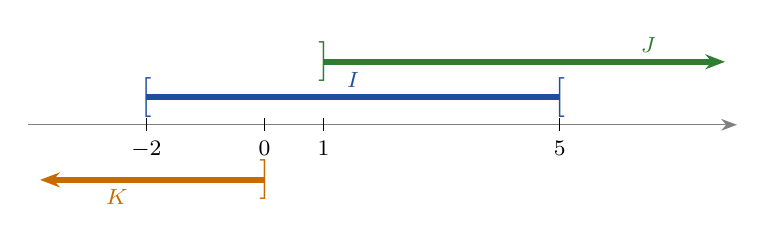
\begin{tikzpicture}[x=0.75cm,font=\footnotesize]
\draw[-{Stealth[length=2mm]},gray] (-4,0)--(8,0);
\foreach \t in {-2,0,1,5}{\draw (\t,0.08)--(\t,-0.08); \node[below] at (\t,-0.08){$\t$};}
\draw[line width=2pt,cDef] (-2,0.35)--(5,0.35); \node[cDef,font=\Large] at (-2,0.35){$[$}; \node[cDef,font=\Large] at (5,0.35){$[$}; \node[cDef,above] at (1.5,0.35){$I$};
\draw[line width=2pt,cRem,-{Stealth[length=2.5mm]}] (1,0.8)--(7.8,0.8); \node[cRem,font=\Large] at (1,0.8){$]$}; \node[cRem,above] at (6.5,0.8){$J$};
\draw[line width=2pt,cEx,{Stealth[length=2.5mm]}-] (-3.8,-0.7)--(0,-0.7); \node[cEx,font=\Large] at (0,-0.7){$]$}; \node[cEx,below] at (-2.5,-0.7){$K$};
\end{tikzpicture}
\end{LTR}\end{center}
\textbf{2.} \bx{I\cap J=\,]1;5[} \ ؛ \ \bx{I\cup J=[-2;+\infty[} \ ؛ \ \bx{I\cap K=[-2;0]} \ ؛ \ \bx{J\cap K=\varnothing} \ ؛ \ \bx{I\cup K=\,]-\infty;5[}
\QQ{3} $-3\leqslant x<2$ \quad أي \quad \bx{x\in[-3;2[}
\QQ{4} المجال $[-1;7]$: مركزه $c=\dfrac{-1+7}2=3$ ونصف قطره $r=\dfrac{7-(-1)}2=4$ \quad إذن: \quad $x\in[-1;7]\iff\bx{|x-3|\leqslant4}$\par
المجال $]2;6[$: مركزه $c=4$ ونصف قطره $r=2$ \quad إذن: \quad $x\in\,]2;6[\iff\bx{|x-4|<2}$
\end{hal}

\begin{tamrin}{تمرين من اختبار الفصل الأول}
نعتبر المجالين $I=[-6;2]$ و $J=\,]-1;7[$.
\begin{enumerate}
\item مثّل المجالين على مستقيم عددي.
\item عيّن: $I\cap J$ ، $I\cup J$ ، $I\cup\R_-$ و $J\cap\R_+$.
\end{enumerate}
\end{tamrin}
\begin{hal}
\textbf{1.}
\begin{center}\begin{LTR}
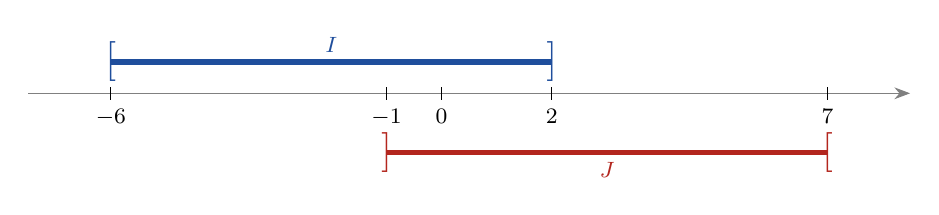
\begin{tikzpicture}[x=0.7cm,font=\footnotesize]
\draw[-{Stealth[length=2mm]},gray] (-7.5,0)--(8.5,0);
\foreach \t in {-6,-1,0,2,7}{\draw (\t,0.08)--(\t,-0.08); \node[below] at (\t,-0.08){$\t$};}
\draw[line width=2pt,cDef] (-6,0.4)--(2,0.4); \node[cDef,font=\Large] at (-6,0.4){$[$}; \node[cDef,font=\Large] at (2,0.4){$]$}; \node[cDef,above] at (-2,0.4){$I$};
\draw[line width=2pt,cThm] (-1,-0.75)--(7,-0.75); \node[cThm,font=\Large] at (-1,-0.75){$]$}; \node[cThm,font=\Large] at (7,-0.75){$[$}; \node[cThm,below] at (3,-0.75){$J$};
\end{tikzpicture}
\end{LTR}\end{center}
\textbf{2.} \bx{I\cap J=\,]-1;2]} \ ؛ \ \bx{I\cup J=[-6;7[} \ ؛ \ \bx{I\cup\R_-=\,]-\infty;2]} \ ؛ \ \bx{J\cap\R_+=[0;7[}
\end{hal}

\begin{tamrin}{تمرين من اختبار الفصل الأول: أكمل الجدول}
أكمل الجدول التالي مع التوضيح:
\begin{center}
\renewcommand{\arraystretch}{1.6}
\begin{tabular}{|>{\centering\arraybackslash}p{0.2\textwidth}|>{\centering\arraybackslash}p{0.2\textwidth}|>{\centering\arraybackslash}p{0.2\textwidth}|>{\centering\arraybackslash}p{0.2\textwidth}|}\hline
\rowcolor{cSec!12}\textbf{القيمة المطلقة} & \textbf{المسافة} & \textbf{الحصر} & \textbf{المجال}\\\hline
$\dots$ & $\dots$ & $\dots$ & $x\in\,]1;3[$\\\hline
$|x+5|<3$ & $\dots$ & $\dots$ & $\dots$\\\hline
$\dots$ & $\dots$ & $\dots$ & $[-3;1]$\\\hline
$\dots$ & $d(x;-3)\leqslant1$ & $\dots$ & $\dots$\\\hline
$\dots$ & $\dots$ & $1\leqslant x\leqslant5$ & $\dots$\\\hline
$\dots$ & $\dots$ & $\dots$ & $[4;8]$\\\hline
$\dots$ & $d\left(x;\frac12\right)<4$ & $\dots$ & $\dots$\\\hline
$\dots$ & $\dots$ & $7\leqslant x\leqslant\frac{15}2$ & $\dots$\\\hline
\end{tabular}
\end{center}
\end{tamrin}
\begin{hal}
\textbf{الطريقة:} نحسب المركز $c=\dfrac{a+b}2$ ونصف القطر $r=\dfrac{b-a}2$ ، ثم نكتب $|x-c|\leqslant r$ (أو $<$ إذا كان المجال مفتوحًا).
\begin{center}
\renewcommand{\arraystretch}{1.6}
\begin{tabular}{|>{\centering\arraybackslash}p{0.2\textwidth}|>{\centering\arraybackslash}p{0.2\textwidth}|>{\centering\arraybackslash}p{0.2\textwidth}|>{\centering\arraybackslash}p{0.2\textwidth}|}\hline
\rowcolor{cSec!12}\textbf{القيمة المطلقة} & \textbf{المسافة} & \textbf{الحصر} & \textbf{المجال}\\\hline
$|x-2|<1$ & $d(x;2)<1$ & $1<x<3$ & $]1;3[$\\\hline
$|x+5|<3$ & $d(x;-5)<3$ & $-8<x<-2$ & $]-8;-2[$\\\hline
$|x+1|\leqslant2$ & $d(x;-1)\leqslant2$ & $-3\leqslant x\leqslant1$ & $[-3;1]$\\\hline
$|x+3|\leqslant1$ & $d(x;-3)\leqslant1$ & $-4\leqslant x\leqslant-2$ & $[-4;-2]$\\\hline
$|x-3|\leqslant2$ & $d(x;3)\leqslant2$ & $1\leqslant x\leqslant5$ & $[1;5]$\\\hline
$|x-6|\leqslant2$ & $d(x;6)\leqslant2$ & $4\leqslant x\leqslant8$ & $[4;8]$\\\hline
$\left|x-\frac12\right|<4$ & $d\left(x;\frac12\right)<4$ & $-\frac72<x<\frac92$ & $\left]-\frac72;\frac92\right[$\\\hline
$\left|x-\frac{29}4\right|\leqslant\frac14$ & $d\left(x;\frac{29}4\right)\leqslant\frac14$ & $7\leqslant x\leqslant\frac{15}2$ & $\left[7;\frac{15}2\right]$\\\hline
\end{tabular}
\end{center}
تفصيل السطر الأخير: \quad $c=\dfrac{7+\frac{15}2}2=\dfrac{29}4$ \quad و \quad $r=\dfrac{\frac{15}2-7}2=\dfrac14$.
\end{hal}

% =====================================================================
\section{القيمة المطلقة والمسافة}
\begin{tamrin}{القيمة المطلقة}
\begin{enumerate}
\item أكتب دون رمز القيمة المطلقة: $A=\left|\sqrt3-2\right|+\left|2\sqrt3-1\right|-\left|\sqrt3-3\right|$.
\item أكتب دون رمز القيمة المطلقة: $B=\left|2-\sqrt5\right|-\left|2\sqrt5-3\right|+\left|7-3\sqrt5\right|$.
\item أكتب دون رمز القيمة المطلقة: $C=\sqrt{\left(\sqrt5-3\right)^2}+\sqrt{\left(\sqrt5-1\right)^2}$.
\end{enumerate}
\end{tamrin}
\begin{hal}
\textbf{1.}
\begin{itemize}
\item $\sqrt3<2$ ، ومنه $\sqrt3-2<0$ \quad و \quad $\left|\sqrt3-2\right|=2-\sqrt3$.
\item $2\sqrt3>1$ ، ومنه $\left|2\sqrt3-1\right|=2\sqrt3-1$.
\item $\sqrt3<3$ ، ومنه $\left|\sqrt3-3\right|=3-\sqrt3$.
\end{itemize}
$A=\left(2-\sqrt3\right)+\left(2\sqrt3-1\right)-\left(3-\sqrt3\right)=\bx{2\sqrt3-2}$
\QQ{2}
\begin{itemize}
\item $\sqrt5>2$: \quad $\left|2-\sqrt5\right|=\sqrt5-2$.
\item $2\sqrt5=\sqrt{20}>3$: \quad $\left|2\sqrt5-3\right|=2\sqrt5-3$.
\item $3\sqrt5=\sqrt{45}<\sqrt{49}=7$: \quad $\left|7-3\sqrt5\right|=7-3\sqrt5$.
\end{itemize}
$B=\left(\sqrt5-2\right)-\left(2\sqrt5-3\right)+\left(7-3\sqrt5\right)=\bx{8-4\sqrt5}$
\QQ{3} $\LW{\sqrt{x^2}=|x|}$: \quad $C=\left|\sqrt5-3\right|+\left|\sqrt5-1\right|=\left(3-\sqrt5\right)+\left(\sqrt5-1\right)=\bx{2}$
\end{hal}

\begin{tamrin}{القيمة المطلقة والمسافة}
\begin{enumerate}
\item اكتب دون رمز القيمة المطلقة: $|\pi-4|$ ، $\left|\sqrt3-2\right|$ ، ثم بسّط $A=\left|\sqrt5-2\right|+\left|\sqrt5-3\right|$.
\item حل في $\R$ المعادلات والمتراجحات التالية:\par
(أ) $|x-2|=5$ \qquad (ب) $|2x+1|=3$ \qquad (جـ) $|x+1|\leqslant3$ \qquad (د) $|x-3|>1$ \qquad (هـ) $|x-1|=|x+3|$
\item نضع $f(x)=|x-1|+|x+2|$. اكتب $f(x)$ دون رمز القيمة المطلقة ، ثم حل المعادلة $f(x)=5$.
\end{enumerate}
\end{tamrin}
\begin{hal}
\textbf{1.} $\pi-4<0$ \quad إذن \quad $|\pi-4|=\bx{4-\pi}$ \qquad ؛ \qquad $\sqrt3<2$ \quad إذن \quad $\left|\sqrt3-2\right|=\bx{2-\sqrt3}$\par
$2<\sqrt5<3$ ، إذن \quad $A=\left(\sqrt5-2\right)+\left(3-\sqrt5\right)=\bx{1}$
\QQ{2}
\begin{itemize}
\item (أ) $|x-2|=5$: المسافة بين $x$ و $2$ تساوي $5$ ، إذن $x=2+5$ أو $x=2-5$ \quad ؛ \quad \bx{S=\{-3;7\}}
\item (ب) $2x+1=3$ أو $2x+1=-3$ ، أي $x=1$ أو $x=-2$ \quad ؛ \quad \bx{S=\{-2;1\}}
\item (جـ) $|x-(-1)|\leqslant3\iff-1-3\leqslant x\leqslant-1+3$ \quad ؛ \quad \bx{S=[-4;2]}
\item (د) المسافة بين $x$ و $3$ أكبر تمامًا من $1$: $x<2$ أو $x>4$ \quad ؛ \quad \bx{S=\,]-\infty;2[\,\cup\,]4;+\infty[}
\item (هـ) $x$ على نفس المسافة من $1$ ومن $-3$ ، إذن $x=\dfrac{1+(-3)}2=-1$ \quad ؛ \quad \bx{S=\{-1\}}
\end{itemize}
\textbf{3.} جدول الإشارة ($x-1$ ينعدم عند $1$ ، و $x+2$ ينعدم عند $-2$):
\begin{center}
\renewcommand{\arraystretch}{1.5}
\begin{tabular}{|c|c|c|c|}\hline
\rowcolor{cSec!12}$[1;+\infty[$ & $[-2;1]$ & $]-\infty;-2]$ & \ar{المجال}\\\hline
$x-1$ & $-x+1$ & $-x+1$ & $|x-1|$\\\hline
$x+2$ & $x+2$ & $-x-2$ & $|x+2|$\\\hline
$2x+1$ & $3$ & $-2x-1$ & $f(x)$\\\hline
\end{tabular}
\end{center}
\begin{itemize}
\item على $]-\infty;-2]$: \quad $-2x-1=5$ \quad ومنه \quad $x=-3$ ، وهو حل مقبول لأن $-3\leqslant-2$.
\item على $[-2;1]$: \quad $3=5$ مستحيلة ، لا حل.
\item على $[1;+\infty[$: \quad $2x+1=5$ \quad ومنه \quad $x=2$ ، وهو حل مقبول لأن $2\geqslant1$.
\end{itemize}
إذن \quad \bx{S=\{-3;2\}}
\end{hal}

\begin{tamrin}{معادلات ومتراجحات تتضمن قيمة مطلقة}
حل في $\R$ المعادلات والمتراجحات التالية:\par
\RL{0.48}{\textbf{1.} $|2x-1|=3$\par \textbf{2.} $|x-4|\leqslant\dfrac52$}{0.48}{\textbf{3.} $|3-x|>1$\par \textbf{4.} $|x+2|\geqslant|x-6|$}
\end{tamrin}
\begin{hal}
\textbf{1.} $|2x-1|=3\iff2x-1=3$ أو $2x-1=-3\iff x=2$ أو $x=-1$ \quad ؛ \quad \bx{S=\{-1;2\}}
\QQ{2} $|x-4|\leqslant\dfrac52\iff4-\dfrac52\leqslant x\leqslant4+\dfrac52\iff\dfrac32\leqslant x\leqslant\dfrac{13}2$ \quad ؛ \quad \bx{S=\left[\frac32;\frac{13}2\right]}
\QQ{3} $|3-x|=|x-3|=d(x;3)>1\iff x<2$ أو $x>4$ \quad ؛ \quad \bx{S=\,]-\infty;2[\,\cup\,]4;+\infty[}
\QQ{4} $d(x;-2)\geqslant d(x;6)$: النقطة $M$ أقرب إلى $6$ أو على نفس البعد. منتصف القطعة: $\dfrac{-2+6}2=2$ ، إذن $x\geqslant2$ \quad ؛ \quad \bx{S=[2;+\infty[}
\end{hal}

\begin{tamrin}{تمارين من اختبارات الفصل الأول}
حل في $\R$ المعادلات والمتراجحات التالية:\par
\RL{0.48}{\textbf{1.} $|x-1|=|x+2|$\par \textbf{2.} $|-x+3|\geqslant4$\par \textbf{3.} $|2x-3|<7$\par \textbf{4.} $|x-2|=5$}{0.48}{\textbf{5.} $|x+3|\leqslant5$\par \textbf{6.} $|x+5|=|x-1|$\par \textbf{7.} $\big||x|-3\big|=|x|-3$\par \textbf{8.} $|x-6|=|x+3|$ (بيانيًا)}
\end{tamrin}
\begin{hal}
\textbf{1.} $d(x;1)=d(x;-2)$: $x$ منتصف $[-2;1]$ ، أي $x=\dfrac{-2+1}2$ \quad ؛ \quad \bx{S=\left\{-\frac12\right\}}
\QQ{2} $|-x+3|=|x-3|\geqslant4\iff x-3\leqslant-4$ أو $x-3\geqslant4\iff x\leqslant-1$ أو $x\geqslant7$ \quad ؛ \quad \bx{S=\,]-\infty;-1]\cup[7;+\infty[}
\QQ{3} $-7<2x-3<7\iff-4<2x<10\iff-2<x<5$ \quad ؛ \quad \bx{S=\,]-2;5[}
\QQ{4} $x-2=5$ أو $x-2=-5$ \quad ؛ \quad \bx{S=\{-3;7\}}
\QQ{5} $-5\leqslant x+3\leqslant5\iff-8\leqslant x\leqslant2$ \quad ؛ \quad \bx{S=[-8;2]}
\QQ{6} $d(x;-5)=d(x;1)$: \quad $x=\dfrac{-5+1}2=-2$ \quad ؛ \quad \bx{S=\{-2\}}
\QQ{7} $|A|=A\iff A\geqslant0$ ، إذن المعادلة تكافئ $|x|-3\geqslant0$ ، أي $|x|\geqslant3$ \quad ؛ \quad \bx{S=\,]-\infty;-3]\cup[3;+\infty[}
\QQ{8} $d(x;6)=d(x;-3)$: $x$ منتصف $[-3;6]$ ، أي \bx{x=\frac32}
\begin{center}\begin{LTR}
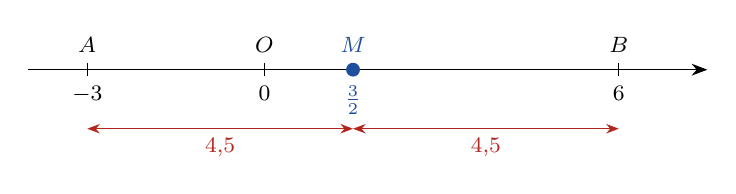
\begin{tikzpicture}[x=0.75cm,font=\footnotesize]
\draw[-{Stealth[length=2mm]}] (-4,0)--(7.5,0);
\foreach \t/\n in {-3/A,0/O,6/B}{\draw (\t,0.08)--(\t,-0.08); \node[below] at (\t,-0.08){$\t$}; \node[above] at (\t,0.1){$\n$};}
\fill[cDef] (1.5,0) circle (2.5pt); \node[above,cDef] at (1.5,0.1){$M$}; \node[below,cDef] at (1.5,-0.08){$\frac32$};
\draw[cThm,{Stealth[length=1.6mm]}-{Stealth[length=1.6mm]}] (-3,-0.75)--(1.5,-0.75) node[midway,below]{$4{,}5$};
\draw[cThm,{Stealth[length=1.6mm]}-{Stealth[length=1.6mm]}] (1.5,-0.75)--(6,-0.75) node[midway,below]{$4{,}5$};
\end{tikzpicture}
\end{LTR}\end{center}
\end{hal}

\begin{tamrin}{تمرين من اختبار الفصل الأول}
حل جبريًا في $\R$ المعادلة: $|2x+5|+|x-9|=12$ (شكّل جدولًا).
\end{tamrin}
\begin{hal}
$2x+5=0\iff x=-\dfrac52$ \quad و \quad $x-9=0\iff x=9$:
\begin{center}
\renewcommand{\arraystretch}{1.5}
\begin{tabular}{|c|c|c|c|}\hline
\rowcolor{cSec!12}$[9;+\infty[$ & $\left[-\frac52;9\right]$ & $\left]-\infty;-\frac52\right]$ & $x$\\\hline
$2x+5$ & $2x+5$ & $-2x-5$ & $|2x+5|$\\\hline
$x-9$ & $-x+9$ & $-x+9$ & $|x-9|$\\\hline
$3x-4$ & $x+14$ & $-3x+4$ & $|2x+5|+|x-9|$\\\hline
\end{tabular}
\end{center}
\begin{itemize}
\item على $\left]-\infty;-\frac52\right]$: \quad $-3x+4=12\iff x=-\dfrac83\approx-2{,}67$ \quad و $-\dfrac83\leqslant-\dfrac52$: \textbf{مقبول}.
\item على $\left[-\frac52;9\right]$: \quad $x+14=12\iff x=-2$ \quad و $-2\in\left[-\frac52;9\right]$: \textbf{مقبول}.
\item على $[9;+\infty[$: \quad $3x-4=12\iff x=\dfrac{16}3\approx5{,}33<9$: \textbf{مرفوض}.
\end{itemize}
إذن \quad \bx{S=\left\{-\frac83;-2\right\}}
\end{hal}

% =====================================================================
\section{تمارين شاملة}
\begin{tamrin}{تمرين من اختبار الفصل الأول}
\textbf{I)} نعتبر العدد الحقيقي $a$ حيث: $a=\sqrt{50}-\sqrt8\left(\sqrt2+1\right)$.
\begin{enumerate}
\item بيّن أن: $a=3\sqrt2-4$ ، ثم استنتج إشارة العدد $a$.
\item نعتبر العددين $x$ و $y$ حيث: $x=\dfrac7{\sqrt2+1}$ و $y=\dfrac1{\sqrt2-1}$.
\begin{sq}
\qa بيّن أن: $x-y=2a$.
\qb استنتج مقارنة العددين $x$ و $y$.
\qc أكتب دون رمز القيمة المطلقة: $|a|$ ، $|y-x|$ و $\left|\dfrac{x-y}2\right|$.
\end{sq}
\end{enumerate}
\textbf{II)} ليكن $z$ عددًا حقيقيًا حيث: $\left|z-\dfrac52\right|\leqslant\dfrac32$.
\begin{enumerate}
\item أثبت أن: $1\leqslant z\leqslant4$.
\item عيّن حصرًا لكل من العددين $\dfrac{\sqrt z}{z+2}$ و $z^2+2z-3$.
\end{enumerate}
\end{tamrin}
\begin{hal}
\textbf{I) 1.} $\sqrt{50}=5\sqrt2$ و $\sqrt8=2\sqrt2$ ، ومنه: \quad $a=5\sqrt2-2\sqrt2\times\sqrt2-2\sqrt2=5\sqrt2-4-2\sqrt2=\bx{3\sqrt2-4}$\par
\textbf{الإشارة:} $3\sqrt2=\sqrt{18}$ و $4=\sqrt{16}$ ، و $\sqrt{18}>\sqrt{16}$ \quad إذن \quad \bx{a>0}
\QQ{2} \pa نضرب في المرافق: \quad $x=\dfrac{7\left(\sqrt2-1\right)}{2-1}=7\sqrt2-7$ \quad و \quad $y=\dfrac{\sqrt2+1}{2-1}=\sqrt2+1$\par
$x-y=7\sqrt2-7-\sqrt2-1=6\sqrt2-8=2\left(3\sqrt2-4\right)=\bx{2a}$
\pb $x-y=2a>0$ \quad إذن \quad \bx{x>y}
\pc $a>0$: \quad $|a|=\bx{3\sqrt2-4}$ \quad ؛ \quad $y-x<0$: \quad $|y-x|=x-y=\bx{6\sqrt2-8}$ \quad ؛ \quad $\left|\dfrac{x-y}2\right|=|a|=\bx{3\sqrt2-4}$
\QQ{\textbf{II) 1}} $\left|z-\dfrac52\right|\leqslant\dfrac32\iff\dfrac52-\dfrac32\leqslant z\leqslant\dfrac52+\dfrac32\iff\bx{1\leqslant z\leqslant4}$
\QQ{2}
\begin{itemize}
\item $1\leqslant\sqrt z\leqslant2$ \quad و \quad $3\leqslant z+2\leqslant6$ ، ومنه $\dfrac16\leqslant\dfrac1{z+2}\leqslant\dfrac13$. بالضرب (أعداد موجبة): \quad \bx{\frac16\leqslant\frac{\sqrt z}{z+2}\leqslant\frac23}
\item $z^2+2z-3=(z+1)^2-4$ ، و $2\leqslant z+1\leqslant5$ ، ومنه $4\leqslant(z+1)^2\leqslant25$ \quad أي \quad \bx{0\leqslant z^2+2z-3\leqslant21}
\end{itemize}
\end{hal}

\begin{tamrin}{تمرين من اختبار الفصل الأول}
لتكن العبارة $P(x)$ حيث: $P(x)=\dfrac12\sqrt{(2x-6)^2}+1$.
\begin{enumerate}
\item بيّن أن: $P(x)=|x-3|+1$.
\item حل في $\R$ المعادلة: $P(x)=2$.
\item أكتب عبارة $P(x)$ دون رمز القيمة المطلقة.
\item
\begin{sq}
\qa تحقق أن: $P\left(\sqrt7\right)=4-\sqrt7$ و $P\left(\sqrt{11}\right)=\sqrt{11}-2$.
\qb استنتج حصرًا لكل من العددين $P\left(\sqrt7\right)$ و $P\left(\sqrt{11}\right)$ إذا علمت أن: $2{,}64<\sqrt7<2{,}65$ و $3{,}31<\sqrt{11}<3{,}32$.
\qc استنتج إشارة الفرق: $P\left(\sqrt{11}\right)-P\left(\sqrt7\right)$.
\end{sq}
\item بيّن أن: $P(x)\leqslant5$ يكافئ $-1\leqslant x\leqslant7$.
\end{enumerate}
\end{tamrin}
\begin{hal}
\textbf{1.} $\sqrt{(2x-6)^2}=|2x-6|=|2(x-3)|=2|x-3|$ \quad ومنه \quad $P(x)=\dfrac12\times2|x-3|+1=\bx{|x-3|+1}$
\QQ{2} $P(x)=2\iff|x-3|=1\iff x-3=1$ أو $x-3=-1\iff x=4$ أو $x=2$ \quad ؛ \quad \bx{S=\{2;4\}}
\QQ{3} \[\bx{P(x)=\begin{cases}x-2 & \text{\ar{إذا كان}}\ x\geqslant3\\ -x+4 & \text{\ar{إذا كان}}\ x\leqslant3\end{cases}}\]
\textbf{4.} \pa $\sqrt7<3$ (لأن $7<9$): \quad $P\left(\sqrt7\right)=-\sqrt7+4$ \ok \qquad ؛ \qquad $\sqrt{11}>3$: \quad $P\left(\sqrt{11}\right)=\sqrt{11}-2$ \ok
\pb $-2{,}65<-\sqrt7<-2{,}64$ \quad ومنه \quad \bx{1{,}35<P\left(\sqrt7\right)<1{,}36} \qquad و \qquad \bx{1{,}31<P\left(\sqrt{11}\right)<1{,}32}
\pc $P\left(\sqrt{11}\right)<1{,}32<1{,}35<P\left(\sqrt7\right)$ \quad إذن \quad \bx{P\left(\sqrt{11}\right)-P\left(\sqrt7\right)<0} (سالب).
\QQ{5} $P(x)\leqslant5\iff|x-3|\leqslant4\iff3-4\leqslant x\leqslant3+4\iff\bx{-1\leqslant x\leqslant7}$
\end{hal}

\begin{tamrin}{تمرين من اختبار الفصل الأول}
\begin{enumerate}
\item لتكن العبارة: $A(x)=|x-6|-2x+7$.
\begin{sq}
\qa أكتب $A(x)$ دون رمز القيمة المطلقة.
\qb عيّن قيم العدد الحقيقي $x$ التي تحقق $A(x)=0$.
\end{sq}
\item نعتبر المستقيم $(d)$ المزود بالمعلم $(O;\vec i)$ ، و $B$ و $C$ نقطتان من $(d)$ فاصلتاهما $-1$ و $5$ ، و $M$ نقطة متحركة فاصلتها $x$.
\begin{sq}
\qa علّم النقطتين $B$ و $C$.
\qb عيّن موضع النقطة $M$ عندما تحقق فاصلتها المعادلة: $|x+1|=|x-5|$.
\end{sq}
\item نعتبر المجموعات: $I=\,]-5;5[$ ، و $J$ مجموعة الأعداد الحقيقية $x$ التي تحقق $|x-5|\leqslant|x+1|$ ، و $K$ مجموعة الأعداد الحقيقية التي تحقق $-6<3x<9$.\par
جد كلًا من $J$ و $K$ ، ثم عيّن: $I\cup(J\cap K)$ ، $I\cap K$ و $J\cup K$.
\end{enumerate}
\end{tamrin}
\begin{hal}
\textbf{1.} \pa
\[\bx{A(x)=\begin{cases}(x-6)-2x+7=-x+1 & \text{\ar{إذا كان}}\ x\geqslant6\\ -(x-6)-2x+7=-3x+13 & \text{\ar{إذا كان}}\ x\leqslant6\end{cases}}\]
\pb إذا كان $x\geqslant6$: \quad $-x+1=0\iff x=1$ ، و $1<6$: \textbf{مرفوض}.\par
إذا كان $x\leqslant6$: \quad $-3x+13=0\iff x=\dfrac{13}3\approx4{,}33\leqslant6$: \textbf{مقبول}. \quad إذن \quad \bx{S=\left\{\frac{13}3\right\}}
\QQ{2} \pa
\begin{center}\begin{LTR}
\begin{tikzpicture}[x=0.8cm,font=\footnotesize]
\draw[-{Stealth[length=2mm]}] (-2.5,0)--(7,0);
\foreach \t/\n in {-1/B,0/O,5/C}{\draw (\t,0.08)--(\t,-0.08); \node[below] at (\t,-0.08){$\t$}; \node[above] at (\t,0.1){$\n$};}
\draw (1,0.08)--(1,-0.08); \node[below] at (1,-0.08){$1$};
\fill[cDef] (2,0) circle (2.5pt); \node[above,cDef] at (2,0.1){$M$}; \node[below,cDef] at (2,-0.08){$2$};
\end{tikzpicture}
\end{LTR}\end{center}
\pb $|x+1|=|x-5|\iff BM=CM$ ، إذن $M$ منتصف $[BC]$: \quad $x=\dfrac{-1+5}2=\bx{2}$
\QQ{3}
\begin{itemize}
\item $J$: $|x-5|\leqslant|x+1|\iff CM\leqslant BM$ ، أي $M$ أقرب إلى $C$ أو على نفس البعد: $x\geqslant2$ \quad ومنه \quad \bx{J=[2;+\infty[}
\item $K$: $-6<3x<9\iff-2<x<3$ \quad ومنه \quad \bx{K=\,]-2;3[}
\item $J\cap K=[2;3[$ ، ومنه \bx{I\cup(J\cap K)=\,]-5;5[} \ ؛ \ \bx{I\cap K=\,]-2;3[} \ ؛ \ \bx{J\cup K=\,]-2;+\infty[}
\end{itemize}
\end{hal}

\begin{tamrin}{تمرين من اختبار الفصل الأول}
نعتبر العبارة: $H(x)=3|x+2|+|2x-4|$.
\begin{enumerate}
\item أحسب كلًا من: $H(2)$ و $H\left(\sqrt6\right)$.
\item أكتب $H(x)$ دون رمز القيمة المطلقة.
\item عيّن قيم $x$ بحيث: $-2\leqslant x\leqslant3$ و $H(x)\geqslant5$.
\end{enumerate}
\end{tamrin}
\begin{hal}
\textbf{1.} $H(2)=3\times4+0=\bx{12}$ \qquad ؛ \qquad $\sqrt6>2$ \quad ومنه \quad $H\left(\sqrt6\right)=3\left(\sqrt6+2\right)+2\sqrt6-4=\bx{5\sqrt6+2}$
\QQ{2} $x+2=0\iff x=-2$ \quad و \quad $2x-4=0\iff x=2$:
\begin{center}
\renewcommand{\arraystretch}{1.5}
\begin{tabular}{|c|c|c|c|}\hline
\rowcolor{cSec!12}$[2;+\infty[$ & $[-2;2]$ & $]-\infty;-2]$ & $x$\\\hline
$3x+6$ & $3x+6$ & $-3x-6$ & $3|x+2|$\\\hline
$2x-4$ & $-2x+4$ & $-2x+4$ & $|2x-4|$\\\hline
$5x+2$ & $x+10$ & $-5x-2$ & $H(x)$\\\hline
\end{tabular}
\end{center}
\textbf{3.}
\begin{itemize}
\item على $[-2;2[$: \quad $x+10\geqslant5\iff x\geqslant-5$: محققة من أجل كل $x\in[-2;2[$.
\item على $[2;3]$: \quad $5x+2\geqslant5\iff x\geqslant\dfrac35$: محققة من أجل كل $x\in[2;3]$.
\end{itemize}
إذن \quad \bx{S=[-2;3]}
\end{hal}

\begin{tamrin}{تمرين نموذجي شامل}
نعتبر العبارة: $E(x)=|x-1|+|x+2|$.
\begin{enumerate}
\item أكتب $E(x)$ دون رمز القيمة المطلقة.
\item حل في $\R$ المعادلة: $E(x)=5$.
\item حل في $\R$ المتراجحة: $E(x)\leqslant3$ ، ثم فسّر النتيجة بيانيًا باستعمال المسافة.
\item ليكن $a\in\left[\sqrt2;\sqrt3\right[$ و $b\in\left[1;\dfrac32\right[$. أعط حصرًا لـ $2a^2-4b$ و $\dfrac{a^2-1}{2b+1}$.
\end{enumerate}
\end{tamrin}
\begin{hal}
\textbf{1.}
\begin{center}
\renewcommand{\arraystretch}{1.5}
\begin{tabular}{|c|c|c|c|}\hline
\rowcolor{cSec!12}$[1;+\infty[$ & $[-2;1]$ & $]-\infty;-2]$ & $x$\\\hline
$x-1$ & $-x+1$ & $-x+1$ & $|x-1|$\\\hline
$x+2$ & $x+2$ & $-x-2$ & $|x+2|$\\\hline
$2x+1$ & $3$ & $-2x-1$ & $E(x)$\\\hline
\end{tabular}
\end{center}
\textbf{2.} على $]-\infty;-2]$: \quad $-2x-1=5\iff x=-3$ (مقبول).\par
على $[-2;1]$: \quad $3=5$ مستحيل. \qquad على $[1;+\infty[$: \quad $2x+1=5\iff x=2$ (مقبول). \quad إذن \quad \bx{S=\{-3;2\}}
\QQ{3} على $]-\infty;-2]$: \quad $-2x-1\leqslant3\iff x\geqslant-2$ ، أي $x=-2$.\par
على $[-2;1]$: \quad $3\leqslant3$ محققة. \qquad على $[1;+\infty[$: \quad $2x+1\leqslant3\iff x\leqslant1$ ، أي $x=1$. \quad إذن \quad \bx{S=[-2;1]}\par
\textbf{التفسير:} $E(x)=d(x;1)+d(x;-2)=MA+MB$ حيث $A(1)$ ، $B(-2)$ و $M(x)$. لدينا $AB=3$ ، و $MA+MB=3$ إذا وفقط إذا كانت $M$ على القطعة $[AB]$ ، وإلا فإن $MA+MB>3$.
\begin{center}\begin{LTR}
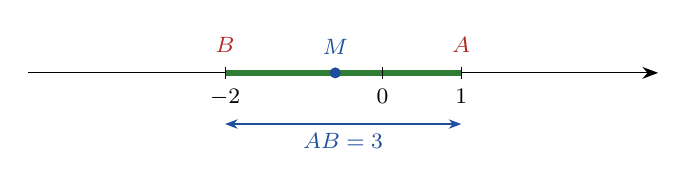
\begin{tikzpicture}[x=1cm,font=\footnotesize]
\draw[-{Stealth[length=2mm]}] (-4.5,0)--(3.5,0);
\draw[line width=2pt,cRem] (-2,0)--(1,0);
\foreach \t in {-2,0,1}{\draw (\t,0.08)--(\t,-0.08); \node[below] at (\t,-0.08){$\t$};}
\node[above=4pt,cThm] at (-2,0){$B$}; \node[above=4pt,cThm] at (1,0){$A$};
\fill[cDef] (-0.6,0) circle (2pt) node[above=3pt]{$M$};
\draw[{Stealth[length=1.6mm]}-{Stealth[length=1.6mm]},cDef] (-2,-0.65)--(1,-0.65) node[midway,below]{$AB=3$};
\end{tikzpicture}
\end{LTR}\end{center}
\textbf{4.}
\begin{itemize}
\item $\sqrt2\leqslant a<\sqrt3$ ، ومنه $2\leqslant a^2<3$ و $4\leqslant2a^2<6$. و $1\leqslant b<\dfrac32$ ، ومنه $-6<-4b\leqslant-4$. بالجمع: \quad \bx{-2<2a^2-4b<2}
\item $1\leqslant a^2-1<2$ ، و $3\leqslant2b+1<4$ ، ومنه $\dfrac14<\dfrac1{2b+1}\leqslant\dfrac13$. بالضرب (أعداد موجبة): \quad \bx{\frac14<\frac{a^2-1}{2b+1}<\frac23}
\end{itemize}
\end{hal}

\begin{tamrin}{تمرين شامل (1)}
نعتبر العددين: $A=\sqrt{45}-\sqrt{20}+\sqrt5$ و $B=\left(1+\sqrt5\right)^2-6$.
\begin{enumerate}
\item اكتب $A$ على الشكل $a\sqrt5$ ، ثم بيّن أن $A=B$.
\item قارن بين $A$ و $4{,}5$ دون استعمال الحاسبة.
\item علمًا أن $2{,}23\leqslant\sqrt5\leqslant2{,}24$ ، أعط حصرًا للعدد $A$ ، ثم مدوّره إلى $10^{-1}$.
\item نضع $C=\dfrac1{A-4}$. اكتب $C$ دون جذر في المقام ، ثم أعط حصرًا له.
\item هل $A$ عدد ناطق؟ علّل.
\end{enumerate}
\end{tamrin}
\begin{hal}
\textbf{1.} $\sqrt{45}=3\sqrt5$ و $\sqrt{20}=2\sqrt5$ \quad إذن \quad $A=3\sqrt5-2\sqrt5+\sqrt5=\bx{2\sqrt5}$\par
$B=1+2\sqrt5+5-6=2\sqrt5$ \quad إذن \quad \bx{A=B}
\QQ{2} $A>0$ و $4{,}5>0$: \quad $A^2=4\times5=20$ \quad و \quad $4{,}5^2=20{,}25$. \quad بما أن $20<20{,}25$ فإن \quad \bx{A<4{,}5}
\QQ{3} بالضرب في $2>0$: \quad \bx{4{,}46\leqslant A\leqslant4{,}48}. كل أعداد هذا المجال مدوّرها إلى $10^{-1}$ هو $4{,}5$ ، إذن مدوّر $A$ إلى $10^{-1}$ هو \bx{4{,}5}.
\QQ{4} $C=\dfrac1{2\sqrt5-4}=\dfrac{2\sqrt5+4}{\left(2\sqrt5-4\right)\left(2\sqrt5+4\right)}=\dfrac{2\sqrt5+4}{20-16}=\dfrac{2\sqrt5+4}4=\bx{\frac{\sqrt5+2}2}$\par
من $2{,}23\leqslant\sqrt5\leqslant2{,}24$: \quad $4{,}23\leqslant\sqrt5+2\leqslant4{,}24$ \quad ومنه \quad \bx{2{,}115\leqslant C\leqslant2{,}12}
\QQ{5} \bxt{لا}. لو كان $A=2\sqrt5=r\in\Q$ لكان $\sqrt5=\dfrac r2\in\Q$ ، وهذا خاطئ لأن $\sqrt5$ عدد أصم (يُبرهن كما في $\sqrt2$ و $\sqrt3$).
\end{hal}

\begin{tamrin}{تمرين شامل (2)}
$x$ عدد حقيقي من المجال $[1;3]$.
\begin{enumerate}
\item أعط حصرًا للعدد $2x-1$ ثم للعدد $\dfrac1{2x-1}$.
\item عبّر عن الشرط $x\in[1;3]$ باستعمال القيمة المطلقة.
\item بسّط العبارة: $E=|x-1|+|x-3|$.
\item نضع: $f(x)=x^2-4x+3$.
\begin{sq}
\qa تحقق أن $f(x)=(x-1)(x-3)$ وأن $f(x)=(x-2)^2-1$.
\qb استنتج أن $-1\leqslant f(x)\leqslant0$ من أجل كل $x\in[1;3]$.
\end{sq}
\end{enumerate}
\end{tamrin}
\begin{hal}
\textbf{1.} $1\leqslant x\leqslant3\Rightarrow2\leqslant2x\leqslant6\Rightarrow\bx{1\leqslant2x-1\leqslant5}$\par
العدد $2x-1$ موجب تمامًا ، والمقلوب يعكس الترتيب: \quad \bx{\frac15\leqslant\frac1{2x-1}\leqslant1}
\QQ{2} مركز المجال $c=\dfrac{1+3}2=2$ ونصف قطره $r=1$ \quad إذن: \quad $x\in[1;3]\iff\bx{|x-2|\leqslant1}$
\QQ{3} على $[1;3]$: $x-1\geqslant0$ و $x-3\leqslant0$ \quad إذن \quad $E=(x-1)+(3-x)=\bx{2}$
\QQ{4} \pa $(x-1)(x-3)=x^2-3x-x+3=x^2-4x+3=f(x)$ \ok \qquad ؛ \qquad $(x-2)^2-1=x^2-4x+4-1=x^2-4x+3=f(x)$ \ok
\pb من السؤال 2: $|x-2|\leqslant1$ ، ومنه $0\leqslant(x-2)^2\leqslant1$ ، وبطرح $1$: \quad $-1\leqslant(x-2)^2-1\leqslant0$ \quad أي \quad \bx{-1\leqslant f(x)\leqslant0}
\end{hal}

\begin{LTR}
\begin{tcolorbox}[enhanced,colback=cSec!10,colframe=cSec!40,arc=3mm,halign=center,boxrule=0.6pt,before upper={\selectlanguage{arabic}}]
{\color{cSec}\Large\bfseries بالتوفيق والنجاح}
\end{tcolorbox}
\end{LTR}
\end{document}
